\documentclass[aspectratio=169]{beamer}

\mode<presentation>
{
  \usetheme{default}
  \usecolortheme{seagull}
  \usefonttheme{serif}
  \setbeamertemplate{navigation symbols}{}
  \setbeamertemplate{caption}[numbered]
  \setbeamertemplate{bibliography item}{}
} 

\usepackage[utf8]{inputenc}
\usepackage[english,russian]{babel}
\usepackage{cmap} % correct output encoding
\usepackage{mathptmx} % russian times new roman
\usepackage[none]{hyphenat} % no word breaks
\sloppy
\hypersetup{unicode=true}

%\setbeamersize{text margin left=1cm, text margin right=1cm} 


%\usepackage{setspace}
%\onehalfspacing

\usepackage{amsmath,amsfonts,amssymb,amsthm,mathtools} % AMS

\usepackage{hyperref}
\hypersetup{
	colorlinks=true,
	linkcolor=black,
	citecolor=black,
	urlcolor=cyan
}

\usepackage{graphicx}
\usepackage{pgf}
\graphicspath{{../text/pics/}}
\DeclareGraphicsExtensions{.pgf,.png}
\usepackage{subfig}

\usepackage{array,tabularx,tabulary,booktabs}
\usepackage{longtable}
\usepackage{multirow}

\usepackage[style=apa,doi=false,backend=biber,natbib]{biblatex}
\addbibresource{ref.bib}

\usepackage[nodayofweek,level]{datetime}
\newcommand{\mydate}{\formatdate{14}{6}{2021}}

\title{Применение гравитационной модели к анализу миграций в Российской империи}
\author{Юрий Соснин, БЭК-182\\Научный руководитель -- Куга Яков Тойвович}
\institute{Высшая Школа Экономики\\Санкт-Петербургская Школа Экономики и Менеджмента}
\date{\mydate}

\newcommand{\btVFill}{\vskip0pt plus 1filll}

\begin{document}

\begin{frame}
  \titlepage
\end{frame}

% \begin{frame}{Оглавление}
%  \tableofcontents
% \end{frame}

\section{Введение}
\begin{frame}{Внутренние миграции: экономическая история}

\begin{figure}
    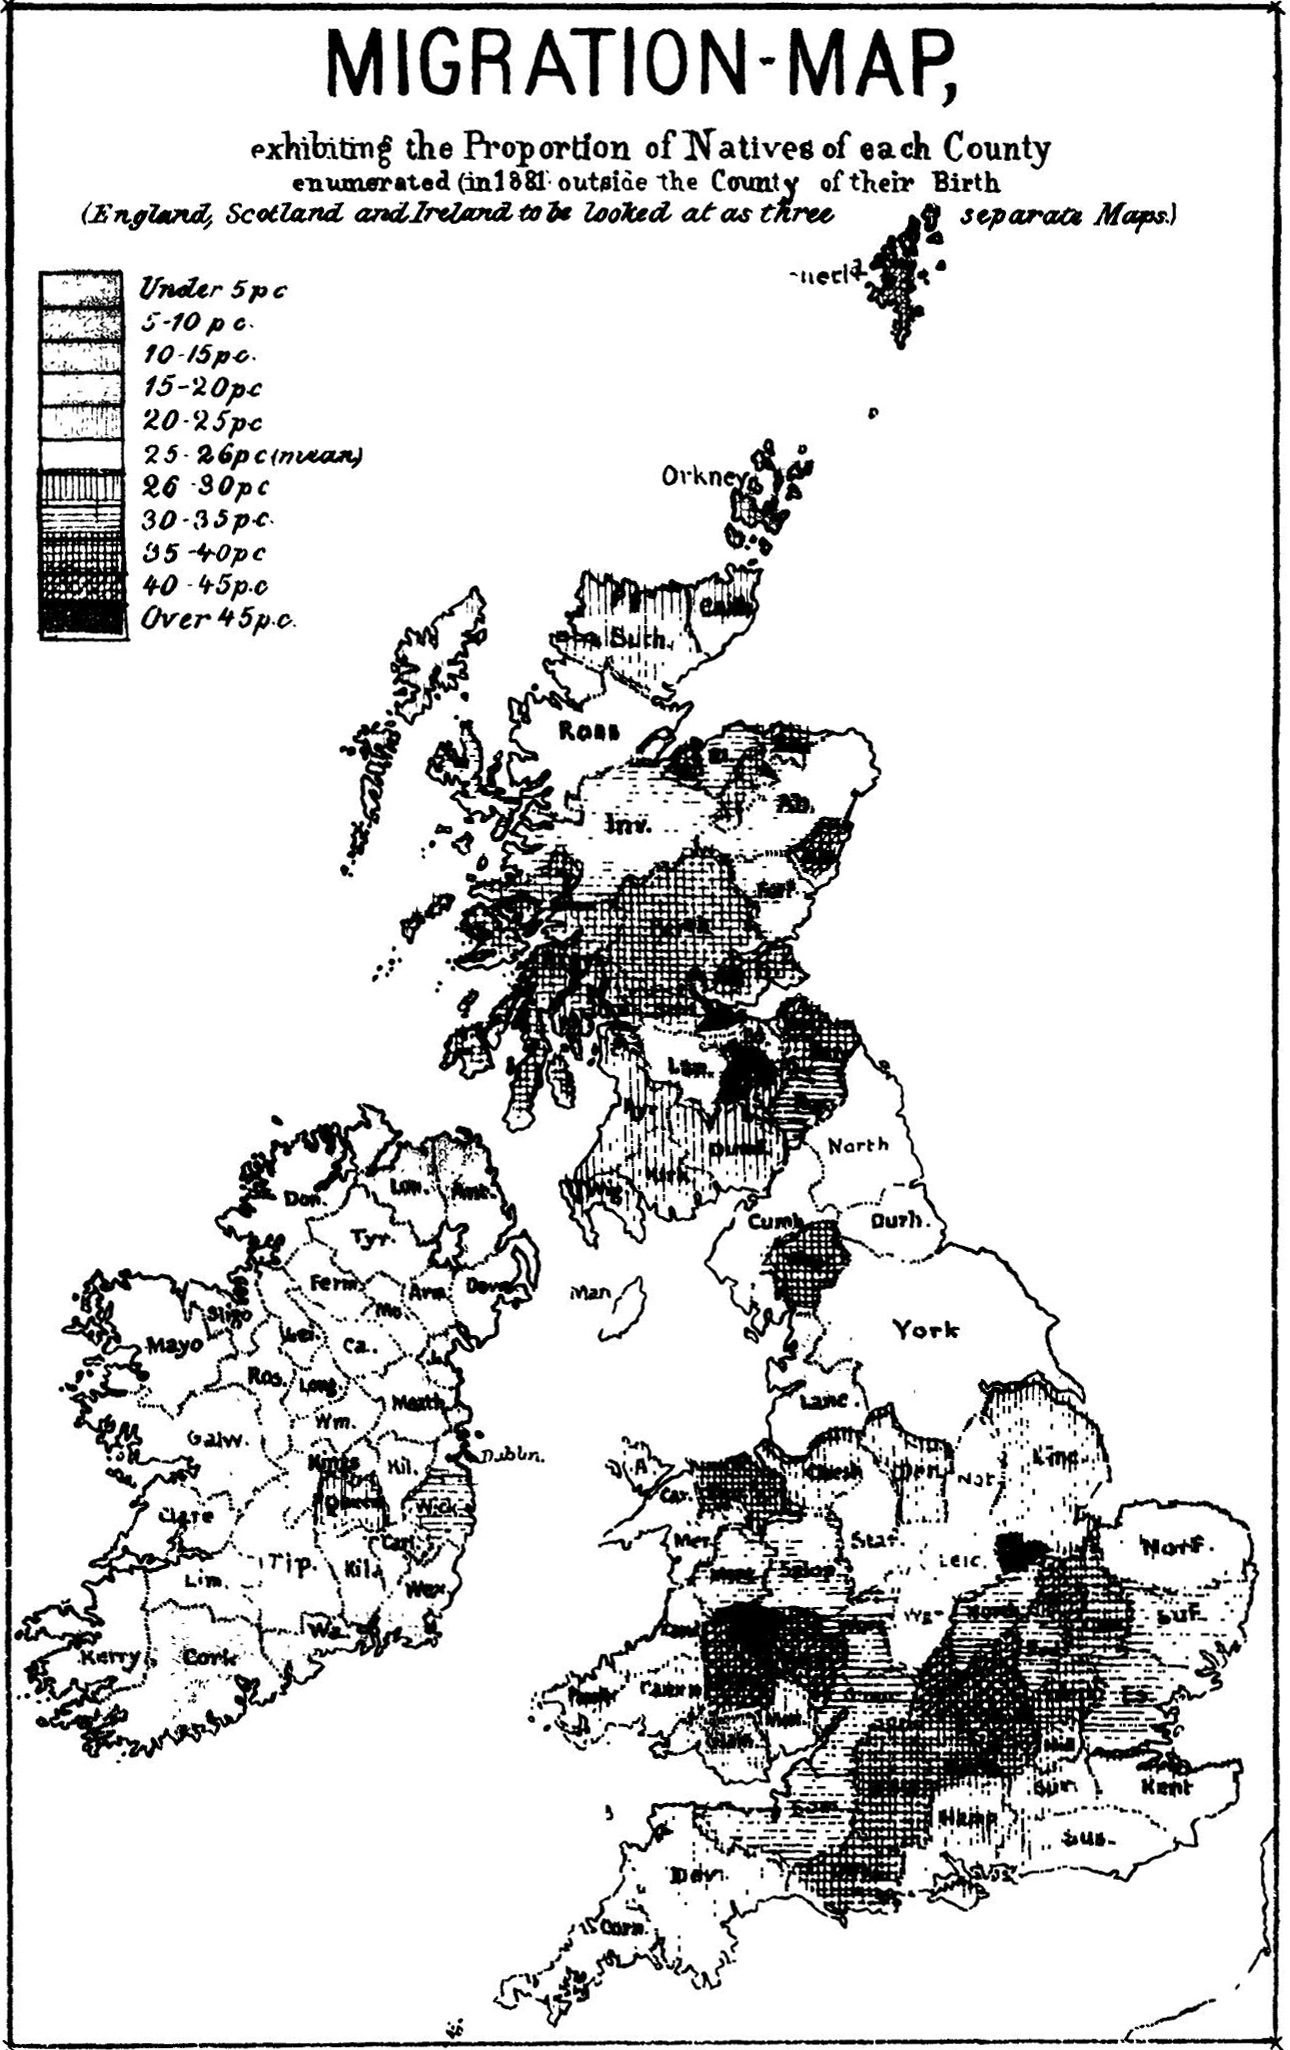
\includegraphics[width=0.28\textwidth]{britain.png}
    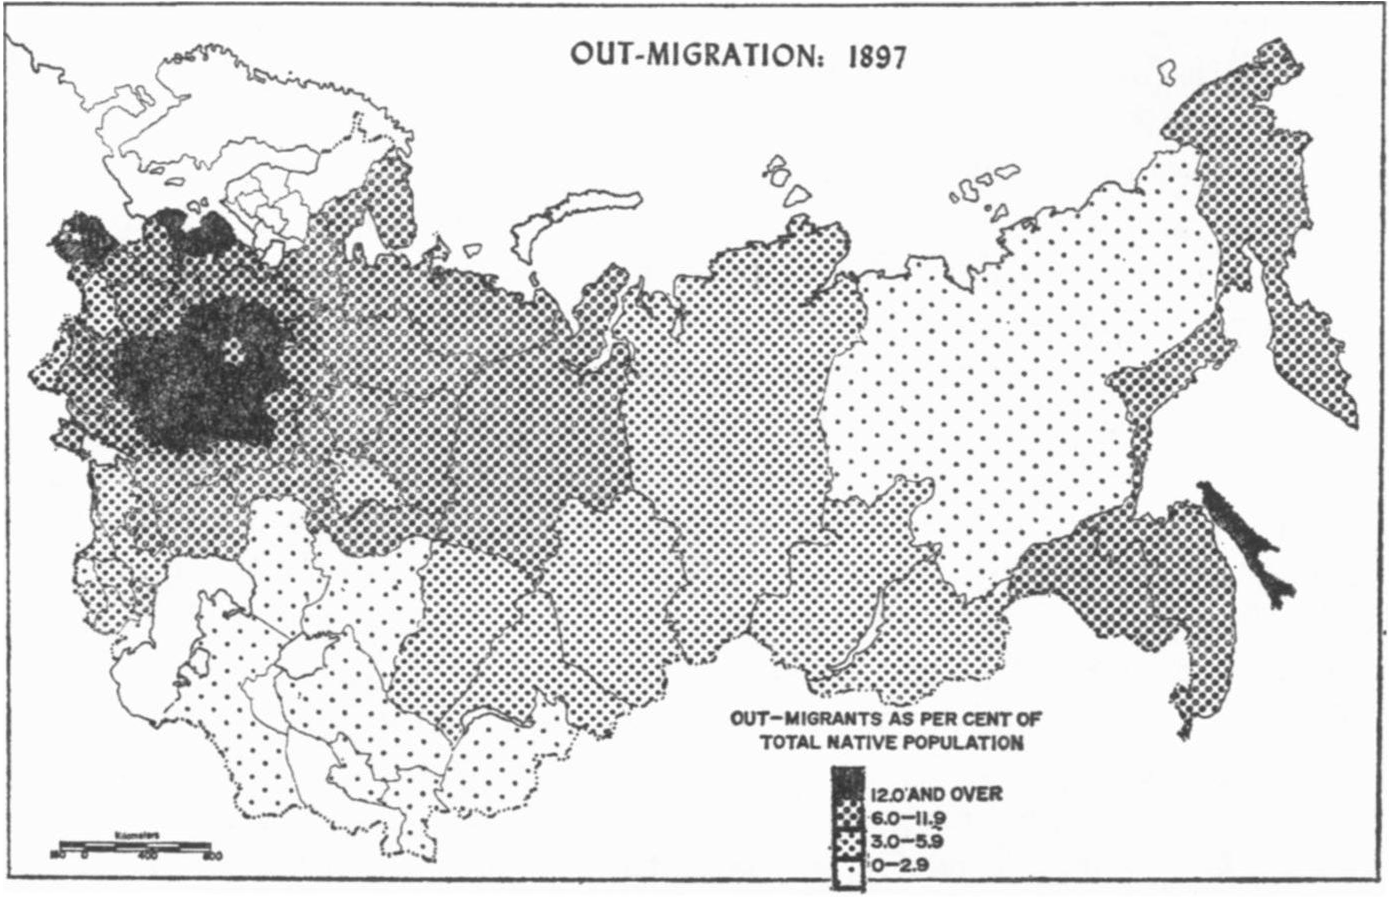
\includegraphics[width=0.68\textwidth]{russia.png}
\end{figure}

\btVFill
\cite{ravenstein_laws_1885}; \cite{leasure_internal_1968}
\bigskip

\end{frame}

\section{Российская империя в 19 веке}
\begin{frame}{Российская империя в 19 веке}

\scalebox{0.9}{%% Creator: Matplotlib, PGF backend
%%
%% To include the figure in your LaTeX document, write
%%   \input{<filename>.pgf}
%%
%% Make sure the required packages are loaded in your preamble
%%   \usepackage{pgf}
%%
%% Figures using additional raster images can only be included by \input if
%% they are in the same directory as the main LaTeX file. For loading figures
%% from other directories you can use the `import` package
%%   \usepackage{import}
%%
%% and then include the figures with
%%   \import{<path to file>}{<filename>.pgf}
%%
%% Matplotlib used the following preamble
%%
\begingroup%
\makeatletter%
\begin{pgfpicture}%
\pgfpathrectangle{\pgfpointorigin}{\pgfqpoint{6.500000in}{3.000000in}}%
\pgfusepath{use as bounding box, clip}%
\begin{pgfscope}%
\pgfsetbuttcap%
\pgfsetmiterjoin%
\pgfsetlinewidth{0.000000pt}%
\definecolor{currentstroke}{rgb}{1.000000,1.000000,1.000000}%
\pgfsetstrokecolor{currentstroke}%
\pgfsetstrokeopacity{0.000000}%
\pgfsetdash{}{0pt}%
\pgfpathmoveto{\pgfqpoint{0.000000in}{0.000000in}}%
\pgfpathlineto{\pgfqpoint{6.500000in}{0.000000in}}%
\pgfpathlineto{\pgfqpoint{6.500000in}{3.000000in}}%
\pgfpathlineto{\pgfqpoint{0.000000in}{3.000000in}}%
\pgfpathclose%
\pgfusepath{}%
\end{pgfscope}%
\begin{pgfscope}%
\pgfsetbuttcap%
\pgfsetmiterjoin%
\definecolor{currentfill}{rgb}{1.000000,1.000000,1.000000}%
\pgfsetfillcolor{currentfill}%
\pgfsetlinewidth{0.000000pt}%
\definecolor{currentstroke}{rgb}{0.000000,0.000000,0.000000}%
\pgfsetstrokecolor{currentstroke}%
\pgfsetstrokeopacity{0.000000}%
\pgfsetdash{}{0pt}%
\pgfpathmoveto{\pgfqpoint{0.812500in}{0.375000in}}%
\pgfpathlineto{\pgfqpoint{4.338750in}{0.375000in}}%
\pgfpathlineto{\pgfqpoint{4.338750in}{2.640000in}}%
\pgfpathlineto{\pgfqpoint{0.812500in}{2.640000in}}%
\pgfpathclose%
\pgfusepath{fill}%
\end{pgfscope}%
\begin{pgfscope}%
\pgfsetbuttcap%
\pgfsetroundjoin%
\definecolor{currentfill}{rgb}{0.000000,0.000000,0.000000}%
\pgfsetfillcolor{currentfill}%
\pgfsetlinewidth{0.803000pt}%
\definecolor{currentstroke}{rgb}{0.000000,0.000000,0.000000}%
\pgfsetstrokecolor{currentstroke}%
\pgfsetdash{}{0pt}%
\pgfsys@defobject{currentmarker}{\pgfqpoint{0.000000in}{-0.048611in}}{\pgfqpoint{0.000000in}{0.000000in}}{%
\pgfpathmoveto{\pgfqpoint{0.000000in}{0.000000in}}%
\pgfpathlineto{\pgfqpoint{0.000000in}{-0.048611in}}%
\pgfusepath{stroke,fill}%
}%
\begin{pgfscope}%
\pgfsys@transformshift{0.972784in}{0.375000in}%
\pgfsys@useobject{currentmarker}{}%
\end{pgfscope}%
\end{pgfscope}%
\begin{pgfscope}%
\definecolor{textcolor}{rgb}{0.000000,0.000000,0.000000}%
\pgfsetstrokecolor{textcolor}%
\pgfsetfillcolor{textcolor}%
\pgftext[x=0.972784in,y=0.277778in,,top]{\color{textcolor}\rmfamily\fontsize{10.000000}{12.000000}\selectfont \(\displaystyle {1885}\)}%
\end{pgfscope}%
\begin{pgfscope}%
\pgfsetbuttcap%
\pgfsetroundjoin%
\definecolor{currentfill}{rgb}{0.000000,0.000000,0.000000}%
\pgfsetfillcolor{currentfill}%
\pgfsetlinewidth{0.803000pt}%
\definecolor{currentstroke}{rgb}{0.000000,0.000000,0.000000}%
\pgfsetstrokecolor{currentstroke}%
\pgfsetdash{}{0pt}%
\pgfsys@defobject{currentmarker}{\pgfqpoint{0.000000in}{-0.048611in}}{\pgfqpoint{0.000000in}{0.000000in}}{%
\pgfpathmoveto{\pgfqpoint{0.000000in}{0.000000in}}%
\pgfpathlineto{\pgfqpoint{0.000000in}{-0.048611in}}%
\pgfusepath{stroke,fill}%
}%
\begin{pgfscope}%
\pgfsys@transformshift{1.545227in}{0.375000in}%
\pgfsys@useobject{currentmarker}{}%
\end{pgfscope}%
\end{pgfscope}%
\begin{pgfscope}%
\definecolor{textcolor}{rgb}{0.000000,0.000000,0.000000}%
\pgfsetstrokecolor{textcolor}%
\pgfsetfillcolor{textcolor}%
\pgftext[x=1.545227in,y=0.277778in,,top]{\color{textcolor}\rmfamily\fontsize{10.000000}{12.000000}\selectfont \(\displaystyle {1890}\)}%
\end{pgfscope}%
\begin{pgfscope}%
\pgfsetbuttcap%
\pgfsetroundjoin%
\definecolor{currentfill}{rgb}{0.000000,0.000000,0.000000}%
\pgfsetfillcolor{currentfill}%
\pgfsetlinewidth{0.803000pt}%
\definecolor{currentstroke}{rgb}{0.000000,0.000000,0.000000}%
\pgfsetstrokecolor{currentstroke}%
\pgfsetdash{}{0pt}%
\pgfsys@defobject{currentmarker}{\pgfqpoint{0.000000in}{-0.048611in}}{\pgfqpoint{0.000000in}{0.000000in}}{%
\pgfpathmoveto{\pgfqpoint{0.000000in}{0.000000in}}%
\pgfpathlineto{\pgfqpoint{0.000000in}{-0.048611in}}%
\pgfusepath{stroke,fill}%
}%
\begin{pgfscope}%
\pgfsys@transformshift{2.117670in}{0.375000in}%
\pgfsys@useobject{currentmarker}{}%
\end{pgfscope}%
\end{pgfscope}%
\begin{pgfscope}%
\definecolor{textcolor}{rgb}{0.000000,0.000000,0.000000}%
\pgfsetstrokecolor{textcolor}%
\pgfsetfillcolor{textcolor}%
\pgftext[x=2.117670in,y=0.277778in,,top]{\color{textcolor}\rmfamily\fontsize{10.000000}{12.000000}\selectfont \(\displaystyle {1895}\)}%
\end{pgfscope}%
\begin{pgfscope}%
\pgfsetbuttcap%
\pgfsetroundjoin%
\definecolor{currentfill}{rgb}{0.000000,0.000000,0.000000}%
\pgfsetfillcolor{currentfill}%
\pgfsetlinewidth{0.803000pt}%
\definecolor{currentstroke}{rgb}{0.000000,0.000000,0.000000}%
\pgfsetstrokecolor{currentstroke}%
\pgfsetdash{}{0pt}%
\pgfsys@defobject{currentmarker}{\pgfqpoint{0.000000in}{-0.048611in}}{\pgfqpoint{0.000000in}{0.000000in}}{%
\pgfpathmoveto{\pgfqpoint{0.000000in}{0.000000in}}%
\pgfpathlineto{\pgfqpoint{0.000000in}{-0.048611in}}%
\pgfusepath{stroke,fill}%
}%
\begin{pgfscope}%
\pgfsys@transformshift{2.690114in}{0.375000in}%
\pgfsys@useobject{currentmarker}{}%
\end{pgfscope}%
\end{pgfscope}%
\begin{pgfscope}%
\definecolor{textcolor}{rgb}{0.000000,0.000000,0.000000}%
\pgfsetstrokecolor{textcolor}%
\pgfsetfillcolor{textcolor}%
\pgftext[x=2.690114in,y=0.277778in,,top]{\color{textcolor}\rmfamily\fontsize{10.000000}{12.000000}\selectfont \(\displaystyle {1900}\)}%
\end{pgfscope}%
\begin{pgfscope}%
\pgfsetbuttcap%
\pgfsetroundjoin%
\definecolor{currentfill}{rgb}{0.000000,0.000000,0.000000}%
\pgfsetfillcolor{currentfill}%
\pgfsetlinewidth{0.803000pt}%
\definecolor{currentstroke}{rgb}{0.000000,0.000000,0.000000}%
\pgfsetstrokecolor{currentstroke}%
\pgfsetdash{}{0pt}%
\pgfsys@defobject{currentmarker}{\pgfqpoint{0.000000in}{-0.048611in}}{\pgfqpoint{0.000000in}{0.000000in}}{%
\pgfpathmoveto{\pgfqpoint{0.000000in}{0.000000in}}%
\pgfpathlineto{\pgfqpoint{0.000000in}{-0.048611in}}%
\pgfusepath{stroke,fill}%
}%
\begin{pgfscope}%
\pgfsys@transformshift{3.262557in}{0.375000in}%
\pgfsys@useobject{currentmarker}{}%
\end{pgfscope}%
\end{pgfscope}%
\begin{pgfscope}%
\definecolor{textcolor}{rgb}{0.000000,0.000000,0.000000}%
\pgfsetstrokecolor{textcolor}%
\pgfsetfillcolor{textcolor}%
\pgftext[x=3.262557in,y=0.277778in,,top]{\color{textcolor}\rmfamily\fontsize{10.000000}{12.000000}\selectfont \(\displaystyle {1905}\)}%
\end{pgfscope}%
\begin{pgfscope}%
\pgfsetbuttcap%
\pgfsetroundjoin%
\definecolor{currentfill}{rgb}{0.000000,0.000000,0.000000}%
\pgfsetfillcolor{currentfill}%
\pgfsetlinewidth{0.803000pt}%
\definecolor{currentstroke}{rgb}{0.000000,0.000000,0.000000}%
\pgfsetstrokecolor{currentstroke}%
\pgfsetdash{}{0pt}%
\pgfsys@defobject{currentmarker}{\pgfqpoint{0.000000in}{-0.048611in}}{\pgfqpoint{0.000000in}{0.000000in}}{%
\pgfpathmoveto{\pgfqpoint{0.000000in}{0.000000in}}%
\pgfpathlineto{\pgfqpoint{0.000000in}{-0.048611in}}%
\pgfusepath{stroke,fill}%
}%
\begin{pgfscope}%
\pgfsys@transformshift{3.835000in}{0.375000in}%
\pgfsys@useobject{currentmarker}{}%
\end{pgfscope}%
\end{pgfscope}%
\begin{pgfscope}%
\definecolor{textcolor}{rgb}{0.000000,0.000000,0.000000}%
\pgfsetstrokecolor{textcolor}%
\pgfsetfillcolor{textcolor}%
\pgftext[x=3.835000in,y=0.277778in,,top]{\color{textcolor}\rmfamily\fontsize{10.000000}{12.000000}\selectfont \(\displaystyle {1910}\)}%
\end{pgfscope}%
\begin{pgfscope}%
\definecolor{textcolor}{rgb}{0.000000,0.000000,0.000000}%
\pgfsetstrokecolor{textcolor}%
\pgfsetfillcolor{textcolor}%
\pgftext[x=2.575625in,y=0.098766in,,top]{\color{textcolor}\rmfamily\fontsize{10.000000}{12.000000}\selectfont Year}%
\end{pgfscope}%
\begin{pgfscope}%
\pgfsetbuttcap%
\pgfsetroundjoin%
\definecolor{currentfill}{rgb}{0.000000,0.000000,0.000000}%
\pgfsetfillcolor{currentfill}%
\pgfsetlinewidth{0.803000pt}%
\definecolor{currentstroke}{rgb}{0.000000,0.000000,0.000000}%
\pgfsetstrokecolor{currentstroke}%
\pgfsetdash{}{0pt}%
\pgfsys@defobject{currentmarker}{\pgfqpoint{-0.048611in}{0.000000in}}{\pgfqpoint{-0.000000in}{0.000000in}}{%
\pgfpathmoveto{\pgfqpoint{-0.000000in}{0.000000in}}%
\pgfpathlineto{\pgfqpoint{-0.048611in}{0.000000in}}%
\pgfusepath{stroke,fill}%
}%
\begin{pgfscope}%
\pgfsys@transformshift{0.812500in}{0.834660in}%
\pgfsys@useobject{currentmarker}{}%
\end{pgfscope}%
\end{pgfscope}%
\begin{pgfscope}%
\definecolor{textcolor}{rgb}{0.000000,0.000000,0.000000}%
\pgfsetstrokecolor{textcolor}%
\pgfsetfillcolor{textcolor}%
\pgftext[x=0.537808in, y=0.786435in, left, base]{\color{textcolor}\rmfamily\fontsize{10.000000}{12.000000}\selectfont \(\displaystyle {7.0}\)}%
\end{pgfscope}%
\begin{pgfscope}%
\pgfsetbuttcap%
\pgfsetroundjoin%
\definecolor{currentfill}{rgb}{0.000000,0.000000,0.000000}%
\pgfsetfillcolor{currentfill}%
\pgfsetlinewidth{0.803000pt}%
\definecolor{currentstroke}{rgb}{0.000000,0.000000,0.000000}%
\pgfsetstrokecolor{currentstroke}%
\pgfsetdash{}{0pt}%
\pgfsys@defobject{currentmarker}{\pgfqpoint{-0.048611in}{0.000000in}}{\pgfqpoint{-0.000000in}{0.000000in}}{%
\pgfpathmoveto{\pgfqpoint{-0.000000in}{0.000000in}}%
\pgfpathlineto{\pgfqpoint{-0.048611in}{0.000000in}}%
\pgfusepath{stroke,fill}%
}%
\begin{pgfscope}%
\pgfsys@transformshift{0.812500in}{1.384832in}%
\pgfsys@useobject{currentmarker}{}%
\end{pgfscope}%
\end{pgfscope}%
\begin{pgfscope}%
\definecolor{textcolor}{rgb}{0.000000,0.000000,0.000000}%
\pgfsetstrokecolor{textcolor}%
\pgfsetfillcolor{textcolor}%
\pgftext[x=0.537808in, y=1.336607in, left, base]{\color{textcolor}\rmfamily\fontsize{10.000000}{12.000000}\selectfont \(\displaystyle {7.5}\)}%
\end{pgfscope}%
\begin{pgfscope}%
\pgfsetbuttcap%
\pgfsetroundjoin%
\definecolor{currentfill}{rgb}{0.000000,0.000000,0.000000}%
\pgfsetfillcolor{currentfill}%
\pgfsetlinewidth{0.803000pt}%
\definecolor{currentstroke}{rgb}{0.000000,0.000000,0.000000}%
\pgfsetstrokecolor{currentstroke}%
\pgfsetdash{}{0pt}%
\pgfsys@defobject{currentmarker}{\pgfqpoint{-0.048611in}{0.000000in}}{\pgfqpoint{-0.000000in}{0.000000in}}{%
\pgfpathmoveto{\pgfqpoint{-0.000000in}{0.000000in}}%
\pgfpathlineto{\pgfqpoint{-0.048611in}{0.000000in}}%
\pgfusepath{stroke,fill}%
}%
\begin{pgfscope}%
\pgfsys@transformshift{0.812500in}{1.935003in}%
\pgfsys@useobject{currentmarker}{}%
\end{pgfscope}%
\end{pgfscope}%
\begin{pgfscope}%
\definecolor{textcolor}{rgb}{0.000000,0.000000,0.000000}%
\pgfsetstrokecolor{textcolor}%
\pgfsetfillcolor{textcolor}%
\pgftext[x=0.537808in, y=1.886778in, left, base]{\color{textcolor}\rmfamily\fontsize{10.000000}{12.000000}\selectfont \(\displaystyle {8.0}\)}%
\end{pgfscope}%
\begin{pgfscope}%
\pgfsetbuttcap%
\pgfsetroundjoin%
\definecolor{currentfill}{rgb}{0.000000,0.000000,0.000000}%
\pgfsetfillcolor{currentfill}%
\pgfsetlinewidth{0.803000pt}%
\definecolor{currentstroke}{rgb}{0.000000,0.000000,0.000000}%
\pgfsetstrokecolor{currentstroke}%
\pgfsetdash{}{0pt}%
\pgfsys@defobject{currentmarker}{\pgfqpoint{-0.048611in}{0.000000in}}{\pgfqpoint{-0.000000in}{0.000000in}}{%
\pgfpathmoveto{\pgfqpoint{-0.000000in}{0.000000in}}%
\pgfpathlineto{\pgfqpoint{-0.048611in}{0.000000in}}%
\pgfusepath{stroke,fill}%
}%
\begin{pgfscope}%
\pgfsys@transformshift{0.812500in}{2.485175in}%
\pgfsys@useobject{currentmarker}{}%
\end{pgfscope}%
\end{pgfscope}%
\begin{pgfscope}%
\definecolor{textcolor}{rgb}{0.000000,0.000000,0.000000}%
\pgfsetstrokecolor{textcolor}%
\pgfsetfillcolor{textcolor}%
\pgftext[x=0.537808in, y=2.436950in, left, base]{\color{textcolor}\rmfamily\fontsize{10.000000}{12.000000}\selectfont \(\displaystyle {8.5}\)}%
\end{pgfscope}%
\begin{pgfscope}%
\definecolor{textcolor}{rgb}{0.000000,0.000000,0.000000}%
\pgfsetstrokecolor{textcolor}%
\pgfsetfillcolor{textcolor}%
\pgftext[x=0.482252in,y=1.507500in,,bottom,rotate=90.000000]{\color{textcolor}\rmfamily\fontsize{10.000000}{12.000000}\selectfont Log of GDP per capita in 1990 dollars}%
\end{pgfscope}%
\begin{pgfscope}%
\pgfpathrectangle{\pgfqpoint{0.812500in}{0.375000in}}{\pgfqpoint{3.526250in}{2.265000in}}%
\pgfusepath{clip}%
\pgfsetrectcap%
\pgfsetroundjoin%
\pgfsetlinewidth{1.505625pt}%
\definecolor{currentstroke}{rgb}{0.121569,0.466667,0.705882}%
\pgfsetstrokecolor{currentstroke}%
\pgfsetdash{}{0pt}%
\pgfpathmoveto{\pgfqpoint{0.972784in}{1.608210in}}%
\pgfpathlineto{\pgfqpoint{1.087273in}{1.634229in}}%
\pgfpathlineto{\pgfqpoint{1.201761in}{1.698308in}}%
\pgfpathlineto{\pgfqpoint{1.316250in}{1.686805in}}%
\pgfpathlineto{\pgfqpoint{1.430739in}{1.667206in}}%
\pgfpathlineto{\pgfqpoint{1.545227in}{1.716015in}}%
\pgfpathlineto{\pgfqpoint{1.659716in}{1.744031in}}%
\pgfpathlineto{\pgfqpoint{1.774205in}{1.756692in}}%
\pgfpathlineto{\pgfqpoint{1.888693in}{1.752342in}}%
\pgfpathlineto{\pgfqpoint{2.003182in}{1.803431in}}%
\pgfpathlineto{\pgfqpoint{2.117670in}{1.821176in}}%
\pgfpathlineto{\pgfqpoint{2.232159in}{1.826485in}}%
\pgfpathlineto{\pgfqpoint{2.346648in}{1.838236in}}%
\pgfpathlineto{\pgfqpoint{2.461136in}{1.887498in}}%
\pgfpathlineto{\pgfqpoint{2.575625in}{1.899382in}}%
\pgfpathlineto{\pgfqpoint{2.690114in}{1.897856in}}%
\pgfpathlineto{\pgfqpoint{2.804602in}{1.890962in}}%
\pgfpathlineto{\pgfqpoint{2.919091in}{1.921650in}}%
\pgfpathlineto{\pgfqpoint{3.033580in}{1.920154in}}%
\pgfpathlineto{\pgfqpoint{3.148068in}{1.925752in}}%
\pgfpathlineto{\pgfqpoint{3.262557in}{1.974535in}}%
\pgfpathlineto{\pgfqpoint{3.377045in}{2.004741in}}%
\pgfpathlineto{\pgfqpoint{3.491534in}{2.059482in}}%
\pgfpathlineto{\pgfqpoint{3.606023in}{2.053532in}}%
\pgfpathlineto{\pgfqpoint{3.720511in}{2.038852in}}%
\pgfpathlineto{\pgfqpoint{3.835000in}{2.043544in}}%
\pgfpathlineto{\pgfqpoint{3.949489in}{2.068347in}}%
\pgfpathlineto{\pgfqpoint{4.063977in}{2.113199in}}%
\pgfpathlineto{\pgfqpoint{4.178466in}{2.100570in}}%
\pgfusepath{stroke}%
\end{pgfscope}%
\begin{pgfscope}%
\pgfpathrectangle{\pgfqpoint{0.812500in}{0.375000in}}{\pgfqpoint{3.526250in}{2.265000in}}%
\pgfusepath{clip}%
\pgfsetrectcap%
\pgfsetroundjoin%
\pgfsetlinewidth{1.505625pt}%
\definecolor{currentstroke}{rgb}{1.000000,0.498039,0.054902}%
\pgfsetstrokecolor{currentstroke}%
\pgfsetdash{}{0pt}%
\pgfpathmoveto{\pgfqpoint{0.972784in}{1.608707in}}%
\pgfpathlineto{\pgfqpoint{1.087273in}{1.606221in}}%
\pgfpathlineto{\pgfqpoint{1.201761in}{1.637620in}}%
\pgfpathlineto{\pgfqpoint{1.316250in}{1.669087in}}%
\pgfpathlineto{\pgfqpoint{1.430739in}{1.686805in}}%
\pgfpathlineto{\pgfqpoint{1.545227in}{1.709238in}}%
\pgfpathlineto{\pgfqpoint{1.659716in}{1.695099in}}%
\pgfpathlineto{\pgfqpoint{1.774205in}{1.727664in}}%
\pgfpathlineto{\pgfqpoint{1.888693in}{1.769637in}}%
\pgfpathlineto{\pgfqpoint{2.003182in}{1.783703in}}%
\pgfpathlineto{\pgfqpoint{2.117670in}{1.820357in}}%
\pgfpathlineto{\pgfqpoint{2.232159in}{1.842259in}}%
\pgfpathlineto{\pgfqpoint{2.346648in}{1.856225in}}%
\pgfpathlineto{\pgfqpoint{2.461136in}{1.884797in}}%
\pgfpathlineto{\pgfqpoint{2.575625in}{1.906602in}}%
\pgfpathlineto{\pgfqpoint{2.690114in}{1.936494in}}%
\pgfpathlineto{\pgfqpoint{2.804602in}{1.893648in}}%
\pgfpathlineto{\pgfqpoint{2.919091in}{1.902047in}}%
\pgfpathlineto{\pgfqpoint{3.033580in}{1.944940in}}%
\pgfpathlineto{\pgfqpoint{3.148068in}{1.972039in}}%
\pgfpathlineto{\pgfqpoint{3.262557in}{1.979509in}}%
\pgfpathlineto{\pgfqpoint{3.377045in}{1.996394in}}%
\pgfpathlineto{\pgfqpoint{3.491534in}{2.028390in}}%
\pgfpathlineto{\pgfqpoint{3.606023in}{2.031438in}}%
\pgfpathlineto{\pgfqpoint{3.720511in}{2.038516in}}%
\pgfpathlineto{\pgfqpoint{3.835000in}{2.062774in}}%
\pgfpathlineto{\pgfqpoint{3.949489in}{2.082318in}}%
\pgfpathlineto{\pgfqpoint{4.063977in}{2.119148in}}%
\pgfpathlineto{\pgfqpoint{4.178466in}{2.157200in}}%
\pgfusepath{stroke}%
\end{pgfscope}%
\begin{pgfscope}%
\pgfpathrectangle{\pgfqpoint{0.812500in}{0.375000in}}{\pgfqpoint{3.526250in}{2.265000in}}%
\pgfusepath{clip}%
\pgfsetrectcap%
\pgfsetroundjoin%
\pgfsetlinewidth{1.505625pt}%
\definecolor{currentstroke}{rgb}{0.172549,0.627451,0.172549}%
\pgfsetstrokecolor{currentstroke}%
\pgfsetdash{}{0pt}%
\pgfpathmoveto{\pgfqpoint{0.972784in}{1.604229in}}%
\pgfpathlineto{\pgfqpoint{1.087273in}{1.619085in}}%
\pgfpathlineto{\pgfqpoint{1.201761in}{1.624972in}}%
\pgfpathlineto{\pgfqpoint{1.316250in}{1.634714in}}%
\pgfpathlineto{\pgfqpoint{1.430739in}{1.660120in}}%
\pgfpathlineto{\pgfqpoint{1.545227in}{1.685417in}}%
\pgfpathlineto{\pgfqpoint{1.659716in}{1.711050in}}%
\pgfpathlineto{\pgfqpoint{1.774205in}{1.738308in}}%
\pgfpathlineto{\pgfqpoint{1.888693in}{1.756692in}}%
\pgfpathlineto{\pgfqpoint{2.003182in}{1.795499in}}%
\pgfpathlineto{\pgfqpoint{2.117670in}{1.771352in}}%
\pgfpathlineto{\pgfqpoint{2.232159in}{1.819947in}}%
\pgfpathlineto{\pgfqpoint{2.346648in}{1.800932in}}%
\pgfpathlineto{\pgfqpoint{2.461136in}{1.850262in}}%
\pgfpathlineto{\pgfqpoint{2.575625in}{1.908872in}}%
\pgfpathlineto{\pgfqpoint{2.690114in}{1.895562in}}%
\pgfpathlineto{\pgfqpoint{2.804602in}{1.876264in}}%
\pgfpathlineto{\pgfqpoint{2.919091in}{1.856225in}}%
\pgfpathlineto{\pgfqpoint{3.033580in}{1.878210in}}%
\pgfpathlineto{\pgfqpoint{3.148068in}{1.884411in}}%
\pgfpathlineto{\pgfqpoint{3.262557in}{1.902428in}}%
\pgfpathlineto{\pgfqpoint{3.377045in}{1.920902in}}%
\pgfpathlineto{\pgfqpoint{3.491534in}{1.967390in}}%
\pgfpathlineto{\pgfqpoint{3.606023in}{1.958392in}}%
\pgfpathlineto{\pgfqpoint{3.720511in}{2.001618in}}%
\pgfpathlineto{\pgfqpoint{3.835000in}{1.929097in}}%
\pgfpathlineto{\pgfqpoint{3.949489in}{2.030084in}}%
\pgfpathlineto{\pgfqpoint{4.063977in}{2.116021in}}%
\pgfpathlineto{\pgfqpoint{4.178466in}{2.106903in}}%
\pgfusepath{stroke}%
\end{pgfscope}%
\begin{pgfscope}%
\pgfpathrectangle{\pgfqpoint{0.812500in}{0.375000in}}{\pgfqpoint{3.526250in}{2.265000in}}%
\pgfusepath{clip}%
\pgfsetrectcap%
\pgfsetroundjoin%
\pgfsetlinewidth{1.505625pt}%
\definecolor{currentstroke}{rgb}{0.839216,0.152941,0.156863}%
\pgfsetstrokecolor{currentstroke}%
\pgfsetdash{}{0pt}%
\pgfpathmoveto{\pgfqpoint{0.972784in}{2.215645in}}%
\pgfpathlineto{\pgfqpoint{1.087273in}{2.222488in}}%
\pgfpathlineto{\pgfqpoint{1.201761in}{2.255529in}}%
\pgfpathlineto{\pgfqpoint{1.316250in}{2.294018in}}%
\pgfpathlineto{\pgfqpoint{1.430739in}{2.341713in}}%
\pgfpathlineto{\pgfqpoint{1.545227in}{2.336600in}}%
\pgfpathlineto{\pgfqpoint{1.659716in}{2.326302in}}%
\pgfpathlineto{\pgfqpoint{1.774205in}{2.288677in}}%
\pgfpathlineto{\pgfqpoint{1.888693in}{2.277378in}}%
\pgfpathlineto{\pgfqpoint{2.003182in}{2.337625in}}%
\pgfpathlineto{\pgfqpoint{2.117670in}{2.360679in}}%
\pgfpathlineto{\pgfqpoint{2.232159in}{2.394014in}}%
\pgfpathlineto{\pgfqpoint{2.346648in}{2.396686in}}%
\pgfpathlineto{\pgfqpoint{2.461136in}{2.437179in}}%
\pgfpathlineto{\pgfqpoint{2.575625in}{2.470351in}}%
\pgfpathlineto{\pgfqpoint{2.690114in}{2.450892in}}%
\pgfpathlineto{\pgfqpoint{2.804602in}{2.439515in}}%
\pgfpathlineto{\pgfqpoint{2.919091in}{2.456880in}}%
\pgfpathlineto{\pgfqpoint{3.033580in}{2.434604in}}%
\pgfpathlineto{\pgfqpoint{3.148068in}{2.430611in}}%
\pgfpathlineto{\pgfqpoint{3.262557in}{2.452276in}}%
\pgfpathlineto{\pgfqpoint{3.377045in}{2.477814in}}%
\pgfpathlineto{\pgfqpoint{3.491534in}{2.488133in}}%
\pgfpathlineto{\pgfqpoint{3.606023in}{2.431552in}}%
\pgfpathlineto{\pgfqpoint{3.720511in}{2.445566in}}%
\pgfpathlineto{\pgfqpoint{3.835000in}{2.468761in}}%
\pgfpathlineto{\pgfqpoint{3.949489in}{2.490809in}}%
\pgfpathlineto{\pgfqpoint{4.063977in}{2.501891in}}%
\pgfpathlineto{\pgfqpoint{4.178466in}{2.537045in}}%
\pgfusepath{stroke}%
\end{pgfscope}%
\begin{pgfscope}%
\pgfpathrectangle{\pgfqpoint{0.812500in}{0.375000in}}{\pgfqpoint{3.526250in}{2.265000in}}%
\pgfusepath{clip}%
\pgfsetrectcap%
\pgfsetroundjoin%
\pgfsetlinewidth{1.505625pt}%
\definecolor{currentstroke}{rgb}{0.580392,0.403922,0.741176}%
\pgfsetstrokecolor{currentstroke}%
\pgfsetdash{}{0pt}%
\pgfpathmoveto{\pgfqpoint{0.972784in}{1.407097in}}%
\pgfpathlineto{\pgfqpoint{1.087273in}{1.430698in}}%
\pgfpathlineto{\pgfqpoint{1.201761in}{1.458366in}}%
\pgfpathlineto{\pgfqpoint{1.316250in}{1.452659in}}%
\pgfpathlineto{\pgfqpoint{1.430739in}{1.418370in}}%
\pgfpathlineto{\pgfqpoint{1.545227in}{1.419550in}}%
\pgfpathlineto{\pgfqpoint{1.659716in}{1.434194in}}%
\pgfpathlineto{\pgfqpoint{1.774205in}{1.435358in}}%
\pgfpathlineto{\pgfqpoint{1.888693in}{1.452087in}}%
\pgfpathlineto{\pgfqpoint{2.003182in}{1.458366in}}%
\pgfpathlineto{\pgfqpoint{2.117670in}{1.467436in}}%
\pgfpathlineto{\pgfqpoint{2.232159in}{1.483688in}}%
\pgfpathlineto{\pgfqpoint{2.346648in}{1.485356in}}%
\pgfpathlineto{\pgfqpoint{2.461136in}{1.480903in}}%
\pgfpathlineto{\pgfqpoint{2.575625in}{1.493105in}}%
\pgfpathlineto{\pgfqpoint{2.690114in}{1.521955in}}%
\pgfpathlineto{\pgfqpoint{2.804602in}{1.539544in}}%
\pgfpathlineto{\pgfqpoint{2.919091in}{1.557377in}}%
\pgfpathlineto{\pgfqpoint{3.033580in}{1.567217in}}%
\pgfpathlineto{\pgfqpoint{3.148068in}{1.586132in}}%
\pgfpathlineto{\pgfqpoint{3.262557in}{1.608707in}}%
\pgfpathlineto{\pgfqpoint{3.377045in}{1.645331in}}%
\pgfpathlineto{\pgfqpoint{3.491534in}{1.664377in}}%
\pgfpathlineto{\pgfqpoint{3.606023in}{1.687730in}}%
\pgfpathlineto{\pgfqpoint{3.720511in}{1.696475in}}%
\pgfpathlineto{\pgfqpoint{3.835000in}{1.697392in}}%
\pgfpathlineto{\pgfqpoint{3.949489in}{1.709238in}}%
\pgfpathlineto{\pgfqpoint{4.063977in}{1.710597in}}%
\pgfpathlineto{\pgfqpoint{4.178466in}{1.761024in}}%
\pgfusepath{stroke}%
\end{pgfscope}%
\begin{pgfscope}%
\pgfpathrectangle{\pgfqpoint{0.812500in}{0.375000in}}{\pgfqpoint{3.526250in}{2.265000in}}%
\pgfusepath{clip}%
\pgfsetrectcap%
\pgfsetroundjoin%
\pgfsetlinewidth{1.505625pt}%
\definecolor{currentstroke}{rgb}{0.549020,0.337255,0.294118}%
\pgfsetstrokecolor{currentstroke}%
\pgfsetdash{}{0pt}%
\pgfpathmoveto{\pgfqpoint{0.972784in}{0.567202in}}%
\pgfpathlineto{\pgfqpoint{1.087273in}{0.636616in}}%
\pgfpathlineto{\pgfqpoint{1.201761in}{0.679033in}}%
\pgfpathlineto{\pgfqpoint{1.316250in}{0.617227in}}%
\pgfpathlineto{\pgfqpoint{1.430739in}{0.656851in}}%
\pgfpathlineto{\pgfqpoint{1.545227in}{0.746285in}}%
\pgfpathlineto{\pgfqpoint{1.659716in}{0.683647in}}%
\pgfpathlineto{\pgfqpoint{1.774205in}{0.747372in}}%
\pgfpathlineto{\pgfqpoint{1.888693in}{0.741927in}}%
\pgfpathlineto{\pgfqpoint{2.003182in}{0.856877in}}%
\pgfpathlineto{\pgfqpoint{2.117670in}{0.860803in}}%
\pgfpathlineto{\pgfqpoint{2.232159in}{0.787893in}}%
\pgfpathlineto{\pgfqpoint{2.346648in}{0.799349in}}%
\pgfpathlineto{\pgfqpoint{2.461136in}{0.977813in}}%
\pgfpathlineto{\pgfqpoint{2.575625in}{0.880227in}}%
\pgfpathlineto{\pgfqpoint{2.690114in}{0.915282in}}%
\pgfpathlineto{\pgfqpoint{2.804602in}{0.939264in}}%
\pgfpathlineto{\pgfqpoint{2.919091in}{0.866667in}}%
\pgfpathlineto{\pgfqpoint{3.033580in}{0.927338in}}%
\pgfpathlineto{\pgfqpoint{3.148068in}{0.922717in}}%
\pgfpathlineto{\pgfqpoint{3.262557in}{0.893623in}}%
\pgfpathlineto{\pgfqpoint{3.377045in}{1.019308in}}%
\pgfpathlineto{\pgfqpoint{3.491534in}{1.042810in}}%
\pgfpathlineto{\pgfqpoint{3.606023in}{1.036981in}}%
\pgfpathlineto{\pgfqpoint{3.720511in}{1.022696in}}%
\pgfpathlineto{\pgfqpoint{3.835000in}{1.025231in}}%
\pgfpathlineto{\pgfqpoint{3.949489in}{1.068257in}}%
\pgfpathlineto{\pgfqpoint{4.063977in}{1.090747in}}%
\pgfpathlineto{\pgfqpoint{4.178466in}{1.093129in}}%
\pgfusepath{stroke}%
\end{pgfscope}%
\begin{pgfscope}%
\pgfpathrectangle{\pgfqpoint{0.812500in}{0.375000in}}{\pgfqpoint{3.526250in}{2.265000in}}%
\pgfusepath{clip}%
\pgfsetrectcap%
\pgfsetroundjoin%
\pgfsetlinewidth{1.505625pt}%
\definecolor{currentstroke}{rgb}{0.890196,0.466667,0.760784}%
\pgfsetstrokecolor{currentstroke}%
\pgfsetdash{}{0pt}%
\pgfpathmoveto{\pgfqpoint{0.972784in}{0.788939in}}%
\pgfpathlineto{\pgfqpoint{1.087273in}{0.838033in}}%
\pgfpathlineto{\pgfqpoint{1.201761in}{0.851949in}}%
\pgfpathlineto{\pgfqpoint{1.316250in}{0.855893in}}%
\pgfpathlineto{\pgfqpoint{1.430739in}{0.825964in}}%
\pgfpathlineto{\pgfqpoint{1.545227in}{0.865691in}}%
\pgfpathlineto{\pgfqpoint{1.659716in}{0.837033in}}%
\pgfpathlineto{\pgfqpoint{1.774205in}{0.824952in}}%
\pgfpathlineto{\pgfqpoint{1.888693in}{0.839033in}}%
\pgfpathlineto{\pgfqpoint{2.003182in}{0.816824in}}%
\pgfpathlineto{\pgfqpoint{2.117670in}{0.854909in}}%
\pgfpathlineto{\pgfqpoint{2.232159in}{0.862761in}}%
\pgfpathlineto{\pgfqpoint{2.346648in}{0.917145in}}%
\pgfpathlineto{\pgfqpoint{2.461136in}{0.946539in}}%
\pgfpathlineto{\pgfqpoint{2.575625in}{0.977813in}}%
\pgfpathlineto{\pgfqpoint{2.690114in}{1.023542in}}%
\pgfpathlineto{\pgfqpoint{2.804602in}{0.995293in}}%
\pgfpathlineto{\pgfqpoint{2.919091in}{0.992689in}}%
\pgfpathlineto{\pgfqpoint{3.033580in}{0.998756in}}%
\pgfpathlineto{\pgfqpoint{3.148068in}{1.003930in}}%
\pgfpathlineto{\pgfqpoint{3.262557in}{0.963627in}}%
\pgfpathlineto{\pgfqpoint{3.377045in}{0.961840in}}%
\pgfpathlineto{\pgfqpoint{3.491534in}{0.977813in}}%
\pgfpathlineto{\pgfqpoint{3.606023in}{0.951061in}}%
\pgfpathlineto{\pgfqpoint{3.720511in}{0.941087in}}%
\pgfpathlineto{\pgfqpoint{3.835000in}{0.959155in}}%
\pgfpathlineto{\pgfqpoint{3.949489in}{0.971629in}}%
\pgfpathlineto{\pgfqpoint{4.063977in}{0.984839in}}%
\pgfpathlineto{\pgfqpoint{4.178466in}{0.978694in}}%
\pgfusepath{stroke}%
\end{pgfscope}%
\begin{pgfscope}%
\pgfpathrectangle{\pgfqpoint{0.812500in}{0.375000in}}{\pgfqpoint{3.526250in}{2.265000in}}%
\pgfusepath{clip}%
\pgfsetrectcap%
\pgfsetroundjoin%
\pgfsetlinewidth{1.505625pt}%
\definecolor{currentstroke}{rgb}{0.498039,0.498039,0.498039}%
\pgfsetstrokecolor{currentstroke}%
\pgfsetdash{}{0pt}%
\pgfpathmoveto{\pgfqpoint{0.972784in}{0.573581in}}%
\pgfpathlineto{\pgfqpoint{1.087273in}{0.530781in}}%
\pgfpathlineto{\pgfqpoint{1.201761in}{0.701910in}}%
\pgfpathlineto{\pgfqpoint{1.316250in}{0.659207in}}%
\pgfpathlineto{\pgfqpoint{1.430739in}{0.579923in}}%
\pgfpathlineto{\pgfqpoint{1.545227in}{0.574853in}}%
\pgfpathlineto{\pgfqpoint{1.659716in}{0.477955in}}%
\pgfpathlineto{\pgfqpoint{1.774205in}{0.578658in}}%
\pgfpathlineto{\pgfqpoint{1.888693in}{0.715412in}}%
\pgfpathlineto{\pgfqpoint{2.003182in}{0.856877in}}%
\pgfpathlineto{\pgfqpoint{2.117670in}{0.772075in}}%
\pgfpathlineto{\pgfqpoint{2.232159in}{0.878300in}}%
\pgfpathlineto{\pgfqpoint{2.346648in}{0.859823in}}%
\pgfpathlineto{\pgfqpoint{2.461136in}{0.887902in}}%
\pgfpathlineto{\pgfqpoint{2.575625in}{0.953766in}}%
\pgfpathlineto{\pgfqpoint{2.690114in}{0.930102in}}%
\pgfpathlineto{\pgfqpoint{2.804602in}{0.956464in}}%
\pgfpathlineto{\pgfqpoint{2.919091in}{1.048608in}}%
\pgfpathlineto{\pgfqpoint{3.033580in}{0.969856in}}%
\pgfpathlineto{\pgfqpoint{3.148068in}{1.080362in}}%
\pgfpathlineto{\pgfqpoint{3.262557in}{0.946539in}}%
\pgfpathlineto{\pgfqpoint{3.377045in}{0.896472in}}%
\pgfpathlineto{\pgfqpoint{3.491534in}{0.851949in}}%
\pgfpathlineto{\pgfqpoint{3.606023in}{0.949254in}}%
\pgfpathlineto{\pgfqpoint{3.720511in}{0.990949in}}%
\pgfpathlineto{\pgfqpoint{3.835000in}{1.061746in}}%
\pgfpathlineto{\pgfqpoint{3.949489in}{0.975167in}}%
\pgfpathlineto{\pgfqpoint{4.063977in}{1.060112in}}%
\pgfpathlineto{\pgfqpoint{4.178466in}{1.114343in}}%
\pgfusepath{stroke}%
\end{pgfscope}%
\begin{pgfscope}%
\pgfpathrectangle{\pgfqpoint{0.812500in}{0.375000in}}{\pgfqpoint{3.526250in}{2.265000in}}%
\pgfusepath{clip}%
\pgfsetrectcap%
\pgfsetroundjoin%
\pgfsetlinewidth{1.505625pt}%
\definecolor{currentstroke}{rgb}{0.737255,0.741176,0.133333}%
\pgfsetstrokecolor{currentstroke}%
\pgfsetdash{}{0pt}%
\pgfpathmoveto{\pgfqpoint{0.972784in}{1.990444in}}%
\pgfpathlineto{\pgfqpoint{1.087273in}{1.998487in}}%
\pgfpathlineto{\pgfqpoint{1.201761in}{2.022951in}}%
\pgfpathlineto{\pgfqpoint{1.316250in}{1.994298in}}%
\pgfpathlineto{\pgfqpoint{1.430739in}{2.037508in}}%
\pgfpathlineto{\pgfqpoint{1.545227in}{2.030761in}}%
\pgfpathlineto{\pgfqpoint{1.659716in}{2.054857in}}%
\pgfpathlineto{\pgfqpoint{1.774205in}{2.134650in}}%
\pgfpathlineto{\pgfqpoint{1.888693in}{2.058493in}}%
\pgfpathlineto{\pgfqpoint{2.003182in}{2.005087in}}%
\pgfpathlineto{\pgfqpoint{2.117670in}{2.109741in}}%
\pgfpathlineto{\pgfqpoint{2.232159in}{2.066710in}}%
\pgfpathlineto{\pgfqpoint{2.346648in}{2.146897in}}%
\pgfpathlineto{\pgfqpoint{2.461136in}{2.149937in}}%
\pgfpathlineto{\pgfqpoint{2.575625in}{2.226177in}}%
\pgfpathlineto{\pgfqpoint{2.690114in}{2.236890in}}%
\pgfpathlineto{\pgfqpoint{2.804602in}{2.333007in}}%
\pgfpathlineto{\pgfqpoint{2.919091in}{2.322156in}}%
\pgfpathlineto{\pgfqpoint{3.033580in}{2.354141in}}%
\pgfpathlineto{\pgfqpoint{3.148068in}{2.319556in}}%
\pgfpathlineto{\pgfqpoint{3.262557in}{2.376113in}}%
\pgfpathlineto{\pgfqpoint{3.377045in}{2.475106in}}%
\pgfpathlineto{\pgfqpoint{3.491534in}{2.471938in}}%
\pgfpathlineto{\pgfqpoint{3.606023in}{2.356408in}}%
\pgfpathlineto{\pgfqpoint{3.720511in}{2.461465in}}%
\pgfpathlineto{\pgfqpoint{3.835000in}{2.449736in}}%
\pgfpathlineto{\pgfqpoint{3.949489in}{2.467624in}}%
\pgfpathlineto{\pgfqpoint{4.063977in}{2.501008in}}%
\pgfpathlineto{\pgfqpoint{4.178466in}{2.521993in}}%
\pgfusepath{stroke}%
\end{pgfscope}%
\begin{pgfscope}%
\pgfsetrectcap%
\pgfsetmiterjoin%
\pgfsetlinewidth{0.803000pt}%
\definecolor{currentstroke}{rgb}{0.000000,0.000000,0.000000}%
\pgfsetstrokecolor{currentstroke}%
\pgfsetdash{}{0pt}%
\pgfpathmoveto{\pgfqpoint{0.812500in}{0.375000in}}%
\pgfpathlineto{\pgfqpoint{0.812500in}{2.640000in}}%
\pgfusepath{stroke}%
\end{pgfscope}%
\begin{pgfscope}%
\pgfsetrectcap%
\pgfsetmiterjoin%
\pgfsetlinewidth{0.803000pt}%
\definecolor{currentstroke}{rgb}{0.000000,0.000000,0.000000}%
\pgfsetstrokecolor{currentstroke}%
\pgfsetdash{}{0pt}%
\pgfpathmoveto{\pgfqpoint{4.338750in}{0.375000in}}%
\pgfpathlineto{\pgfqpoint{4.338750in}{2.640000in}}%
\pgfusepath{stroke}%
\end{pgfscope}%
\begin{pgfscope}%
\pgfsetrectcap%
\pgfsetmiterjoin%
\pgfsetlinewidth{0.803000pt}%
\definecolor{currentstroke}{rgb}{0.000000,0.000000,0.000000}%
\pgfsetstrokecolor{currentstroke}%
\pgfsetdash{}{0pt}%
\pgfpathmoveto{\pgfqpoint{0.812500in}{0.375000in}}%
\pgfpathlineto{\pgfqpoint{4.338750in}{0.375000in}}%
\pgfusepath{stroke}%
\end{pgfscope}%
\begin{pgfscope}%
\pgfsetrectcap%
\pgfsetmiterjoin%
\pgfsetlinewidth{0.803000pt}%
\definecolor{currentstroke}{rgb}{0.000000,0.000000,0.000000}%
\pgfsetstrokecolor{currentstroke}%
\pgfsetdash{}{0pt}%
\pgfpathmoveto{\pgfqpoint{0.812500in}{2.640000in}}%
\pgfpathlineto{\pgfqpoint{4.338750in}{2.640000in}}%
\pgfusepath{stroke}%
\end{pgfscope}%
\begin{pgfscope}%
\pgfsetrectcap%
\pgfsetroundjoin%
\pgfsetlinewidth{1.505625pt}%
\definecolor{currentstroke}{rgb}{0.121569,0.466667,0.705882}%
\pgfsetstrokecolor{currentstroke}%
\pgfsetdash{}{0pt}%
\pgfpathmoveto{\pgfqpoint{4.463750in}{2.295694in}}%
\pgfpathlineto{\pgfqpoint{4.741528in}{2.295694in}}%
\pgfusepath{stroke}%
\end{pgfscope}%
\begin{pgfscope}%
\definecolor{textcolor}{rgb}{0.000000,0.000000,0.000000}%
\pgfsetstrokecolor{textcolor}%
\pgfsetfillcolor{textcolor}%
\pgftext[x=4.852639in,y=2.247083in,left,base]{\color{textcolor}\rmfamily\fontsize{10.000000}{12.000000}\selectfont Austria-Hungary}%
\end{pgfscope}%
\begin{pgfscope}%
\pgfsetrectcap%
\pgfsetroundjoin%
\pgfsetlinewidth{1.505625pt}%
\definecolor{currentstroke}{rgb}{1.000000,0.498039,0.054902}%
\pgfsetstrokecolor{currentstroke}%
\pgfsetdash{}{0pt}%
\pgfpathmoveto{\pgfqpoint{4.463750in}{2.102021in}}%
\pgfpathlineto{\pgfqpoint{4.741528in}{2.102021in}}%
\pgfusepath{stroke}%
\end{pgfscope}%
\begin{pgfscope}%
\definecolor{textcolor}{rgb}{0.000000,0.000000,0.000000}%
\pgfsetstrokecolor{textcolor}%
\pgfsetfillcolor{textcolor}%
\pgftext[x=4.852639in,y=2.053410in,left,base]{\color{textcolor}\rmfamily\fontsize{10.000000}{12.000000}\selectfont Germany}%
\end{pgfscope}%
\begin{pgfscope}%
\pgfsetrectcap%
\pgfsetroundjoin%
\pgfsetlinewidth{1.505625pt}%
\definecolor{currentstroke}{rgb}{0.172549,0.627451,0.172549}%
\pgfsetstrokecolor{currentstroke}%
\pgfsetdash{}{0pt}%
\pgfpathmoveto{\pgfqpoint{4.463750in}{1.908349in}}%
\pgfpathlineto{\pgfqpoint{4.741528in}{1.908349in}}%
\pgfusepath{stroke}%
\end{pgfscope}%
\begin{pgfscope}%
\definecolor{textcolor}{rgb}{0.000000,0.000000,0.000000}%
\pgfsetstrokecolor{textcolor}%
\pgfsetfillcolor{textcolor}%
\pgftext[x=4.852639in,y=1.859738in,left,base]{\color{textcolor}\rmfamily\fontsize{10.000000}{12.000000}\selectfont France}%
\end{pgfscope}%
\begin{pgfscope}%
\pgfsetrectcap%
\pgfsetroundjoin%
\pgfsetlinewidth{1.505625pt}%
\definecolor{currentstroke}{rgb}{0.839216,0.152941,0.156863}%
\pgfsetstrokecolor{currentstroke}%
\pgfsetdash{}{0pt}%
\pgfpathmoveto{\pgfqpoint{4.463750in}{1.714676in}}%
\pgfpathlineto{\pgfqpoint{4.741528in}{1.714676in}}%
\pgfusepath{stroke}%
\end{pgfscope}%
\begin{pgfscope}%
\definecolor{textcolor}{rgb}{0.000000,0.000000,0.000000}%
\pgfsetstrokecolor{textcolor}%
\pgfsetfillcolor{textcolor}%
\pgftext[x=4.852639in,y=1.666065in,left,base]{\color{textcolor}\rmfamily\fontsize{10.000000}{12.000000}\selectfont United Kingdom}%
\end{pgfscope}%
\begin{pgfscope}%
\pgfsetrectcap%
\pgfsetroundjoin%
\pgfsetlinewidth{1.505625pt}%
\definecolor{currentstroke}{rgb}{0.580392,0.403922,0.741176}%
\pgfsetstrokecolor{currentstroke}%
\pgfsetdash{}{0pt}%
\pgfpathmoveto{\pgfqpoint{4.463750in}{1.521003in}}%
\pgfpathlineto{\pgfqpoint{4.741528in}{1.521003in}}%
\pgfusepath{stroke}%
\end{pgfscope}%
\begin{pgfscope}%
\definecolor{textcolor}{rgb}{0.000000,0.000000,0.000000}%
\pgfsetstrokecolor{textcolor}%
\pgfsetfillcolor{textcolor}%
\pgftext[x=4.852639in,y=1.472392in,left,base]{\color{textcolor}\rmfamily\fontsize{10.000000}{12.000000}\selectfont Italy}%
\end{pgfscope}%
\begin{pgfscope}%
\pgfsetrectcap%
\pgfsetroundjoin%
\pgfsetlinewidth{1.505625pt}%
\definecolor{currentstroke}{rgb}{0.549020,0.337255,0.294118}%
\pgfsetstrokecolor{currentstroke}%
\pgfsetdash{}{0pt}%
\pgfpathmoveto{\pgfqpoint{4.463750in}{1.327330in}}%
\pgfpathlineto{\pgfqpoint{4.741528in}{1.327330in}}%
\pgfusepath{stroke}%
\end{pgfscope}%
\begin{pgfscope}%
\definecolor{textcolor}{rgb}{0.000000,0.000000,0.000000}%
\pgfsetstrokecolor{textcolor}%
\pgfsetfillcolor{textcolor}%
\pgftext[x=4.852639in,y=1.278719in,left,base]{\color{textcolor}\rmfamily\fontsize{10.000000}{12.000000}\selectfont Japan}%
\end{pgfscope}%
\begin{pgfscope}%
\pgfsetrectcap%
\pgfsetroundjoin%
\pgfsetlinewidth{1.505625pt}%
\definecolor{currentstroke}{rgb}{0.890196,0.466667,0.760784}%
\pgfsetstrokecolor{currentstroke}%
\pgfsetdash{}{0pt}%
\pgfpathmoveto{\pgfqpoint{4.463750in}{1.133657in}}%
\pgfpathlineto{\pgfqpoint{4.741528in}{1.133657in}}%
\pgfusepath{stroke}%
\end{pgfscope}%
\begin{pgfscope}%
\definecolor{textcolor}{rgb}{0.000000,0.000000,0.000000}%
\pgfsetstrokecolor{textcolor}%
\pgfsetfillcolor{textcolor}%
\pgftext[x=4.852639in,y=1.085046in,left,base]{\color{textcolor}\rmfamily\fontsize{10.000000}{12.000000}\selectfont Portugal}%
\end{pgfscope}%
\begin{pgfscope}%
\pgfsetrectcap%
\pgfsetroundjoin%
\pgfsetlinewidth{1.505625pt}%
\definecolor{currentstroke}{rgb}{0.498039,0.498039,0.498039}%
\pgfsetstrokecolor{currentstroke}%
\pgfsetdash{}{0pt}%
\pgfpathmoveto{\pgfqpoint{4.463750in}{0.939985in}}%
\pgfpathlineto{\pgfqpoint{4.741528in}{0.939985in}}%
\pgfusepath{stroke}%
\end{pgfscope}%
\begin{pgfscope}%
\definecolor{textcolor}{rgb}{0.000000,0.000000,0.000000}%
\pgfsetstrokecolor{textcolor}%
\pgfsetfillcolor{textcolor}%
\pgftext[x=4.852639in,y=0.891374in,left,base]{\color{textcolor}\rmfamily\fontsize{10.000000}{12.000000}\selectfont Russia}%
\end{pgfscope}%
\begin{pgfscope}%
\pgfsetrectcap%
\pgfsetroundjoin%
\pgfsetlinewidth{1.505625pt}%
\definecolor{currentstroke}{rgb}{0.737255,0.741176,0.133333}%
\pgfsetstrokecolor{currentstroke}%
\pgfsetdash{}{0pt}%
\pgfpathmoveto{\pgfqpoint{4.463750in}{0.746312in}}%
\pgfpathlineto{\pgfqpoint{4.741528in}{0.746312in}}%
\pgfusepath{stroke}%
\end{pgfscope}%
\begin{pgfscope}%
\definecolor{textcolor}{rgb}{0.000000,0.000000,0.000000}%
\pgfsetstrokecolor{textcolor}%
\pgfsetfillcolor{textcolor}%
\pgftext[x=4.852639in,y=0.697701in,left,base]{\color{textcolor}\rmfamily\fontsize{10.000000}{12.000000}\selectfont United States}%
\end{pgfscope}%
\end{pgfpicture}%
\makeatother%
\endgroup%
}

\btVFill
\cite{gregory_russian_1983}; \cite{maddison_project_2018}
\bigskip

\end{frame}

\begin{frame}{Российская империя в 19 веке}

\begin{columns}
	\begin{column}{0.58\textwidth}
	    \begin{figure}
		    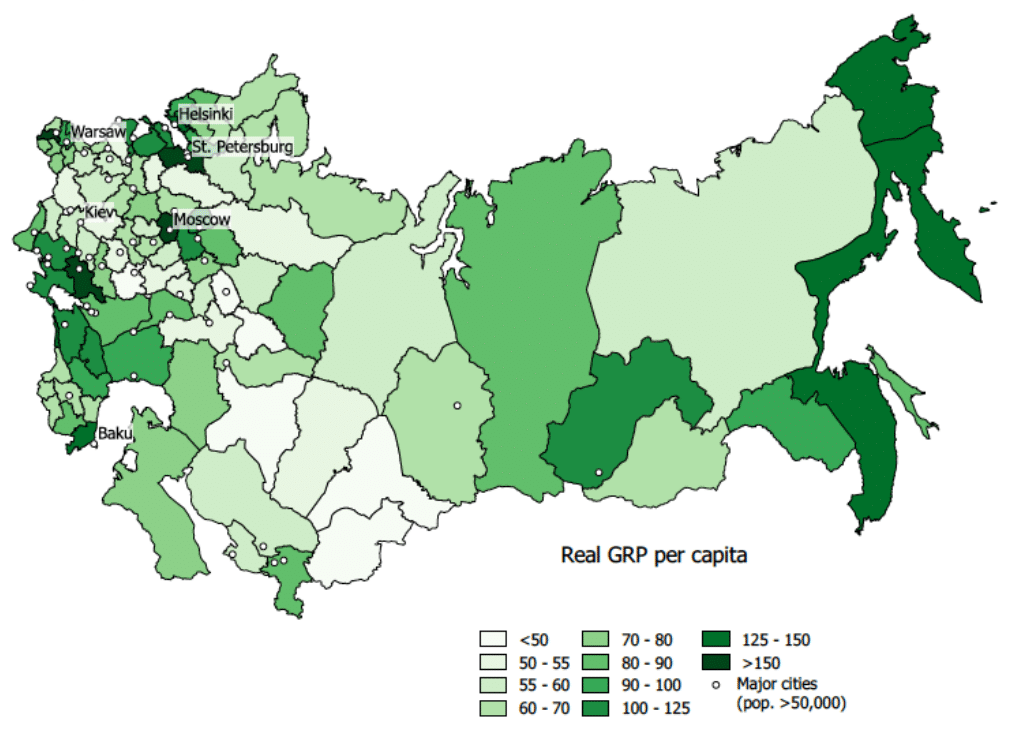
\includegraphics[width=1.05\textwidth]{markevich.png}
	    \end{figure}
	\end{column}
	
	\begin{column}{0.38\textwidth}
	    \begin{table}[h]
	        \caption{Подушевой продукт, 1897, 1990\$}
	        \newcommand{\tableecowidth}{\textwidth}
	        \label{table:eco}
\centering
\begin{tabularx}{\tableecowidth}{Xl}
\hline
Российская империя           & 1122 \\
Санкт-Петербургская губерния & 6826 \\
Тургайская область           & 567  \\
Великобритания               & 4428 \\
США                          & 3780 \\
Португалия                   & 1182 \\
Япония                       & 1062 \\
\hline
\end{tabularx}
        \end{table}
	\end{column}
\end{columns}

\btVFill
\cite{markevich_regional_2019}
\bigskip

\end{frame}

\section{Исследовательский вопрос}
\begin{frame}{Исследовательский вопрос}

Какие характеристики регионов влияли на внутренние миграции в Российской империи конца 19 века?
\par
Я анализирую влияние:
\begin{itemize}
	\item плотности населения и урбанизации
	\item социального развития (грамотности, естественного прироста населения)
	\item уровня индустриализации
\end{itemize}

\end{frame}

\section{Данные}
{
\usebackgroundtemplate{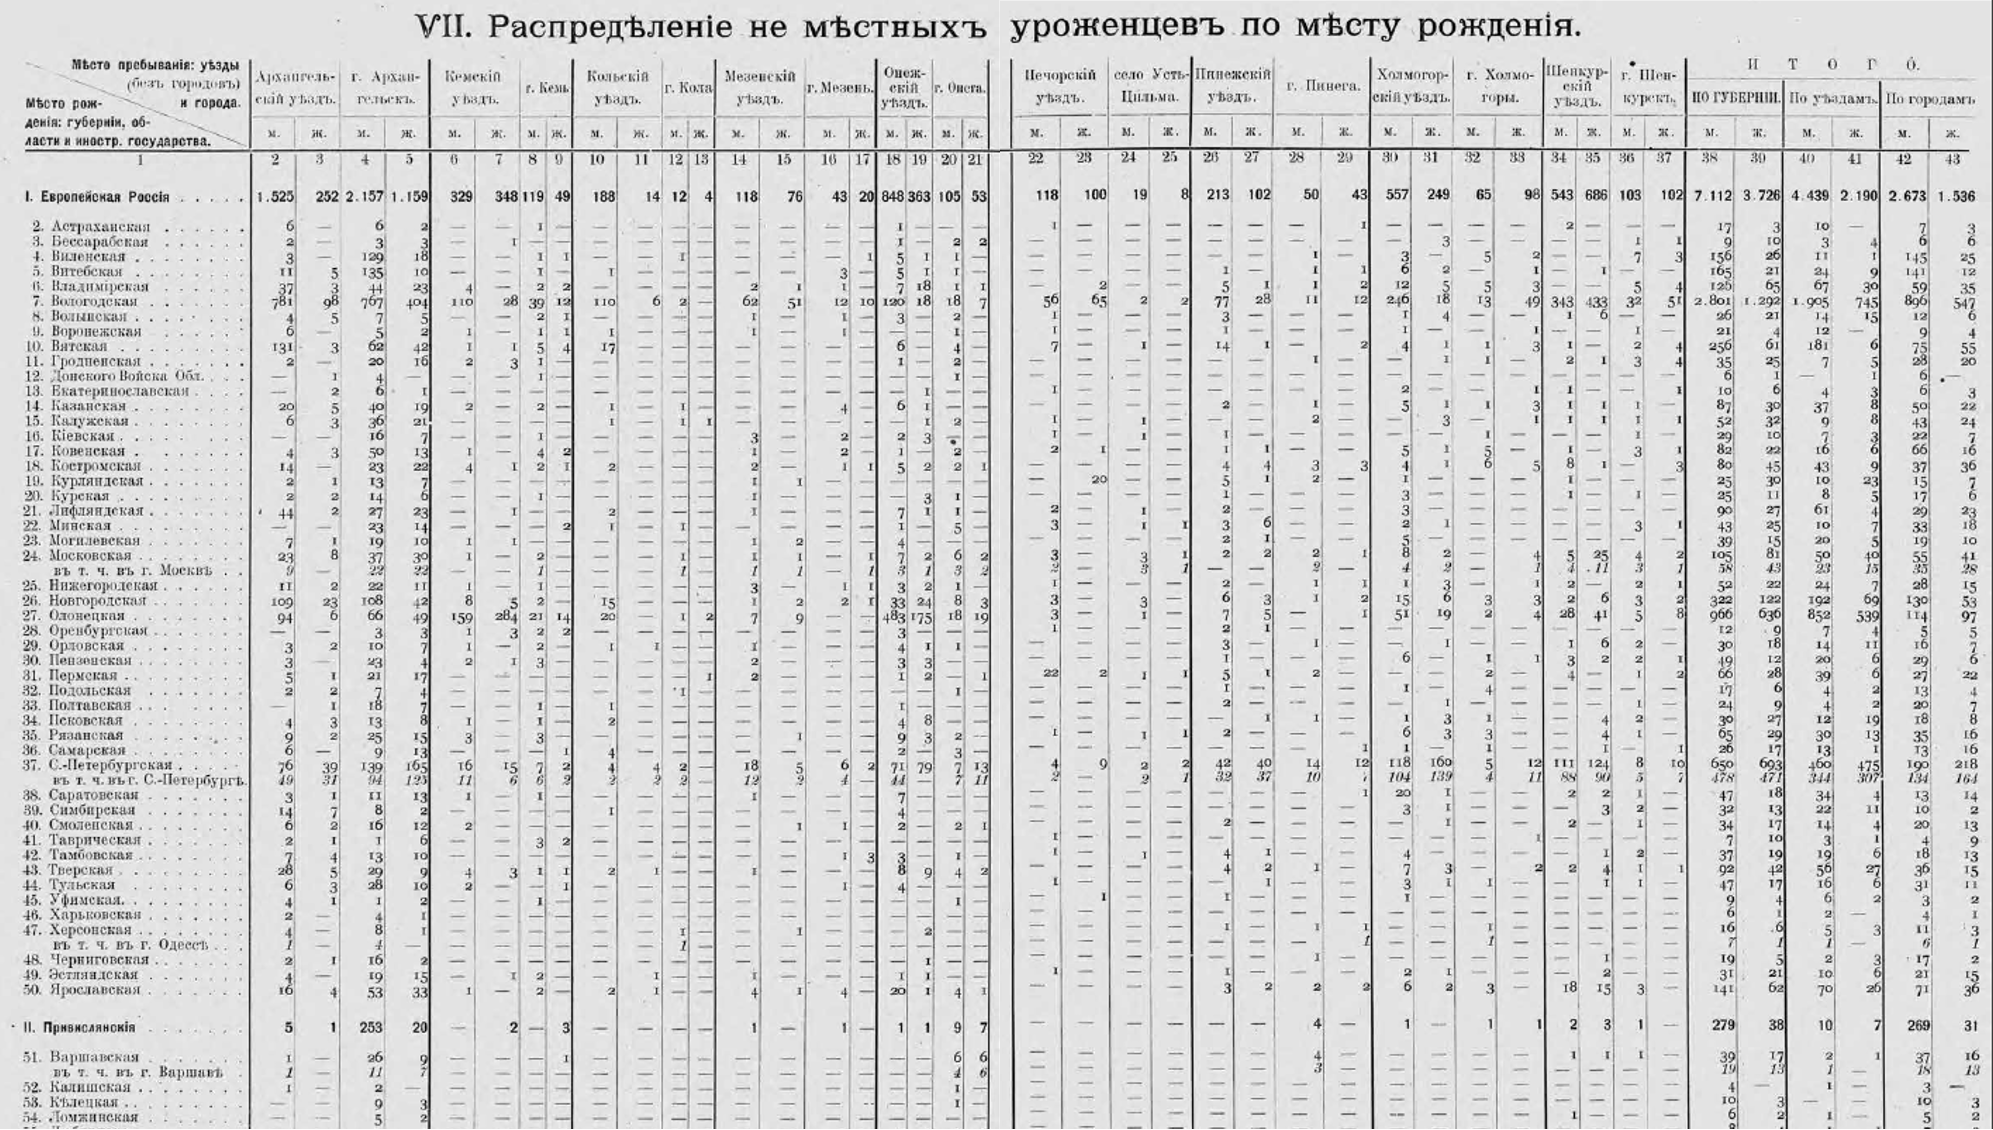
\includegraphics[width=\paperwidth]{census.png}}
\setbeamertemplate{navigation symbols}{}
\begin{frame}[b]
\hfill \colorbox{white}{\parbox{0.64\textwidth}{Первая всеобщая перепись населения \par Российской империи 1897 года \citep{census_1897}}}
\bigskip
\end{frame}
}

\begin{frame}{Недостатки данных}

\begin{itemize}
	\item Один год, кросс-секция
	\item Пожизненная миграция
	\item Нет важных экономических показателей и прочих переменных
\end{itemize}
\par
Ограниченная возможность делать каузальные выводы

\end{frame}

%\begin{frame}{Миграция из регионов}
%	
%\begin{figure}[h!]
%	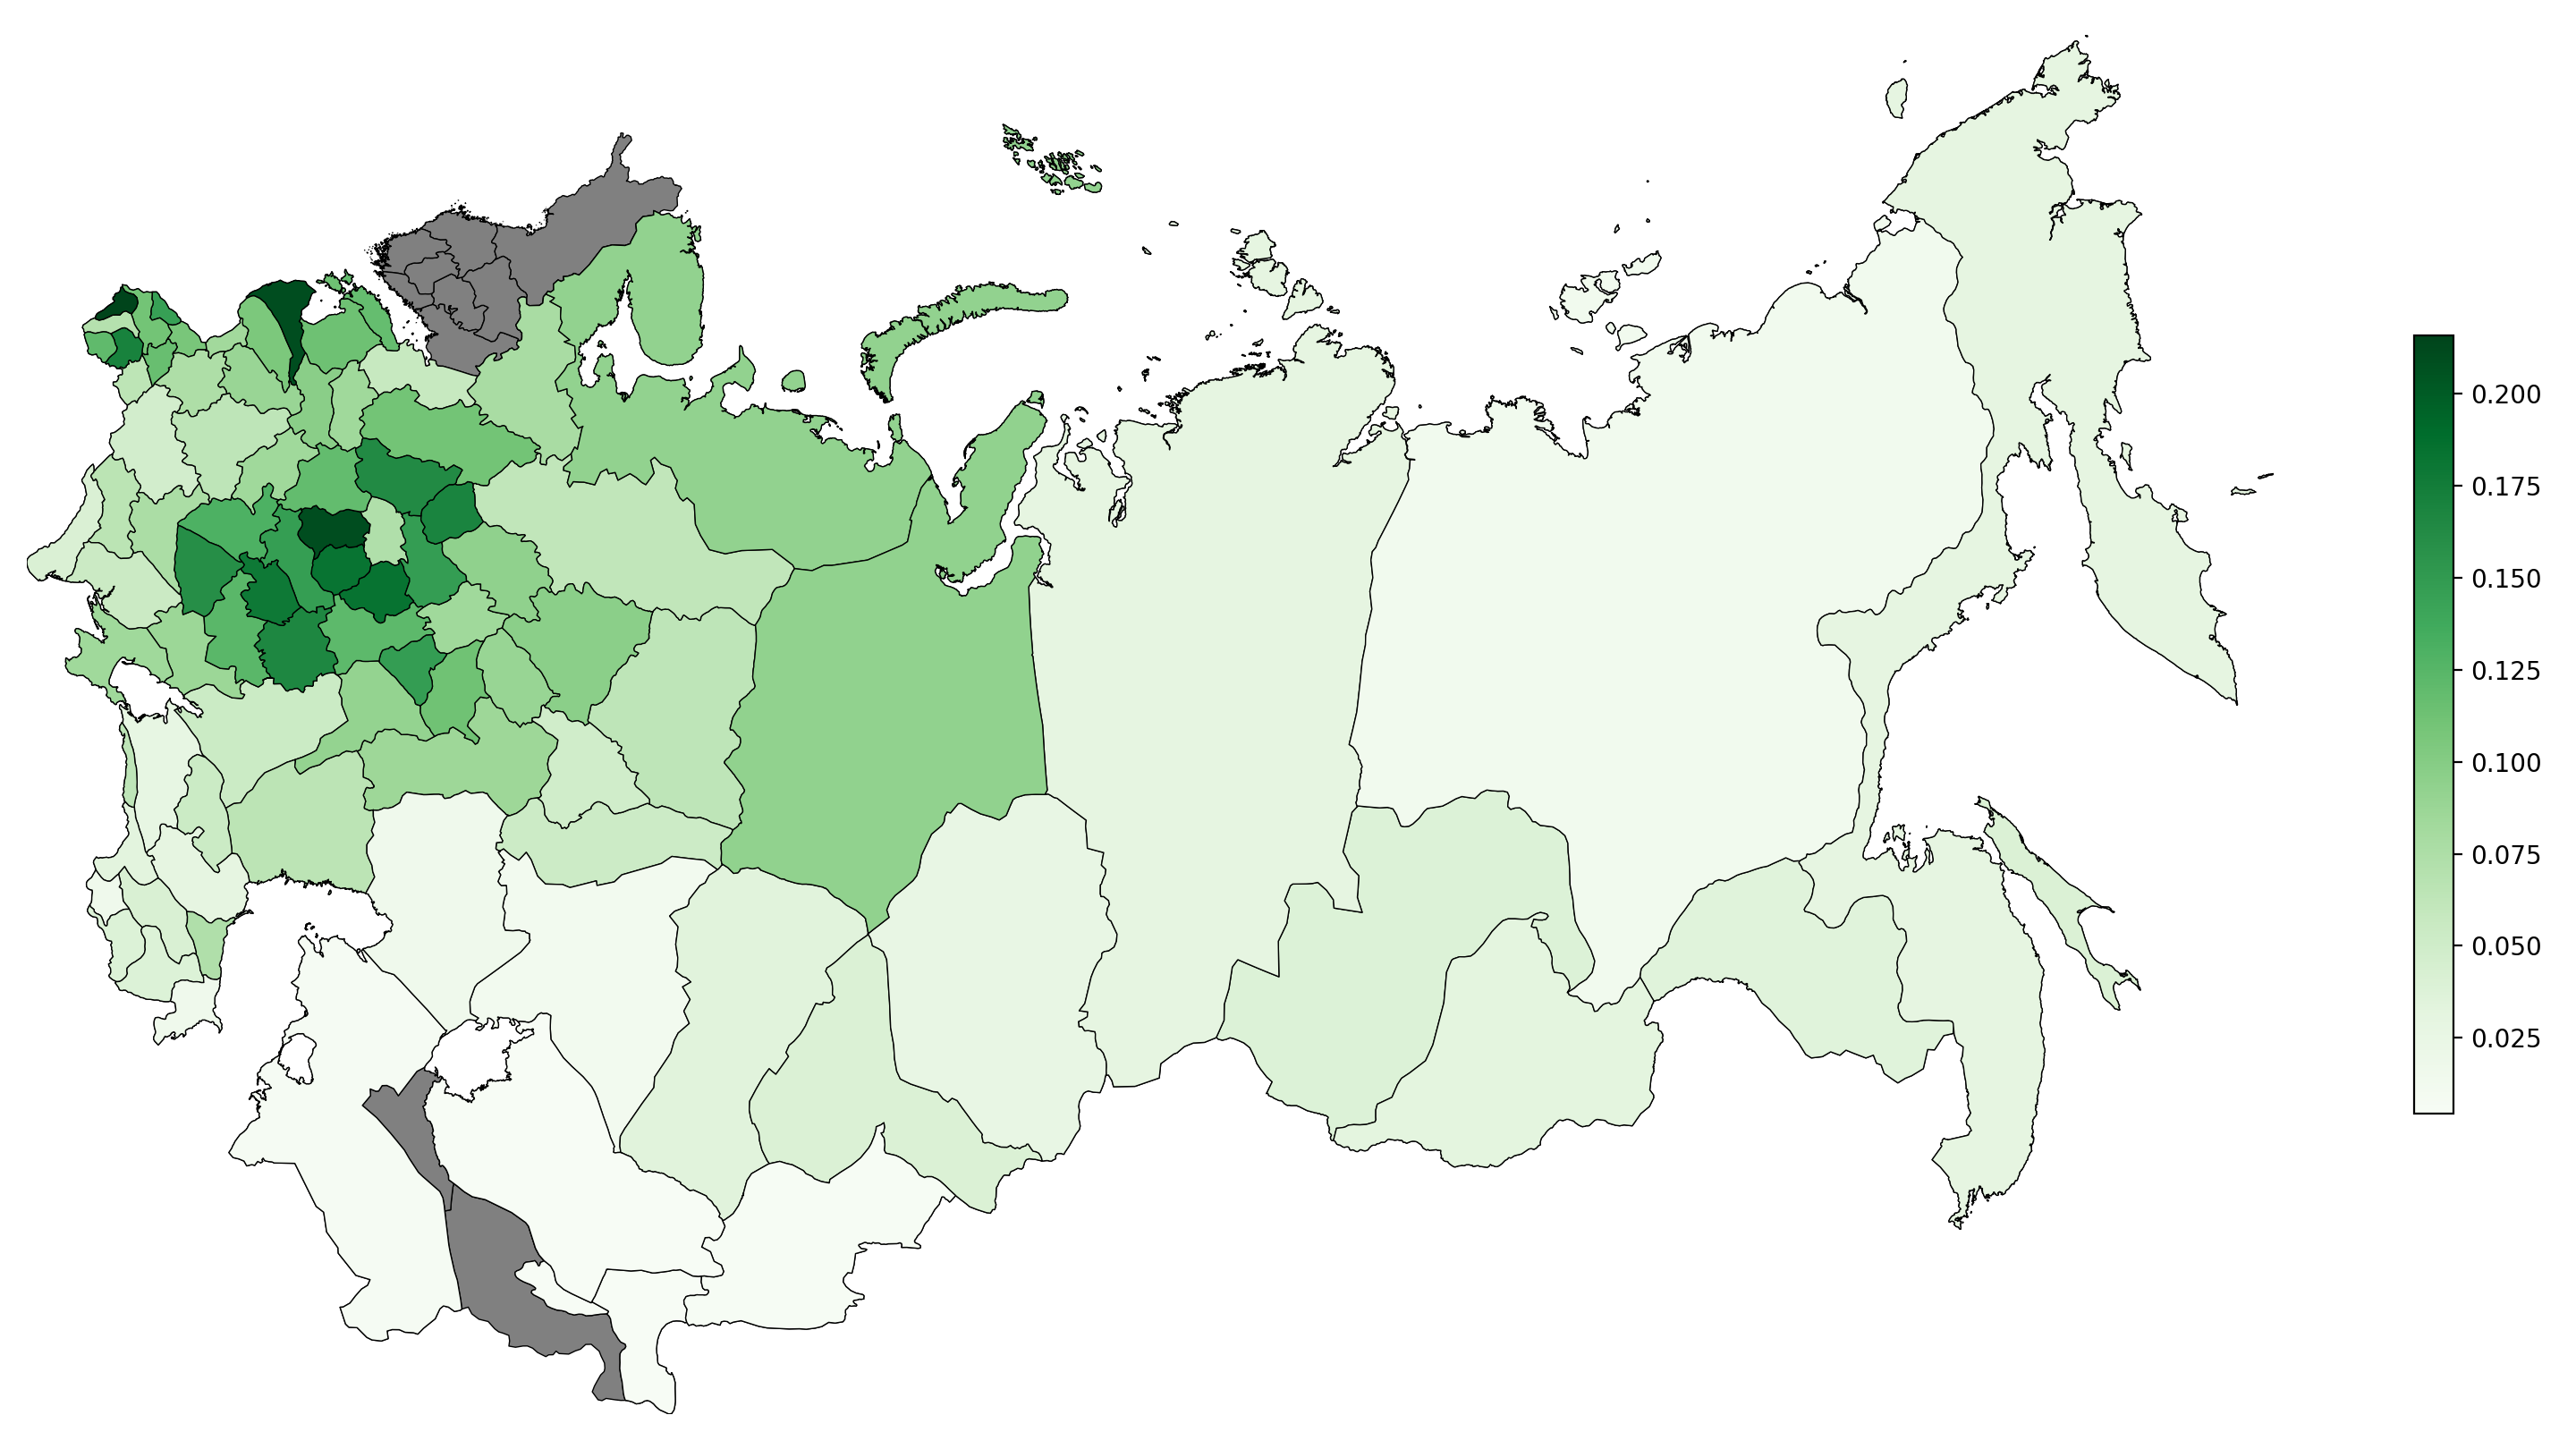
\includegraphics[height=0.85\textheight]{mig_of_pop_from.png}
%\end{figure}
%
%\btVFill
%\hfill \href{https://russia-migrations-1897.herokuapp.com}{russia-migrations-189%7.herokuapp.com}
%\bigskip
%\end{frame}

{
\usebackgroundtemplate{
  \parbox[c][\paperheight][c]{\paperwidth}{\centering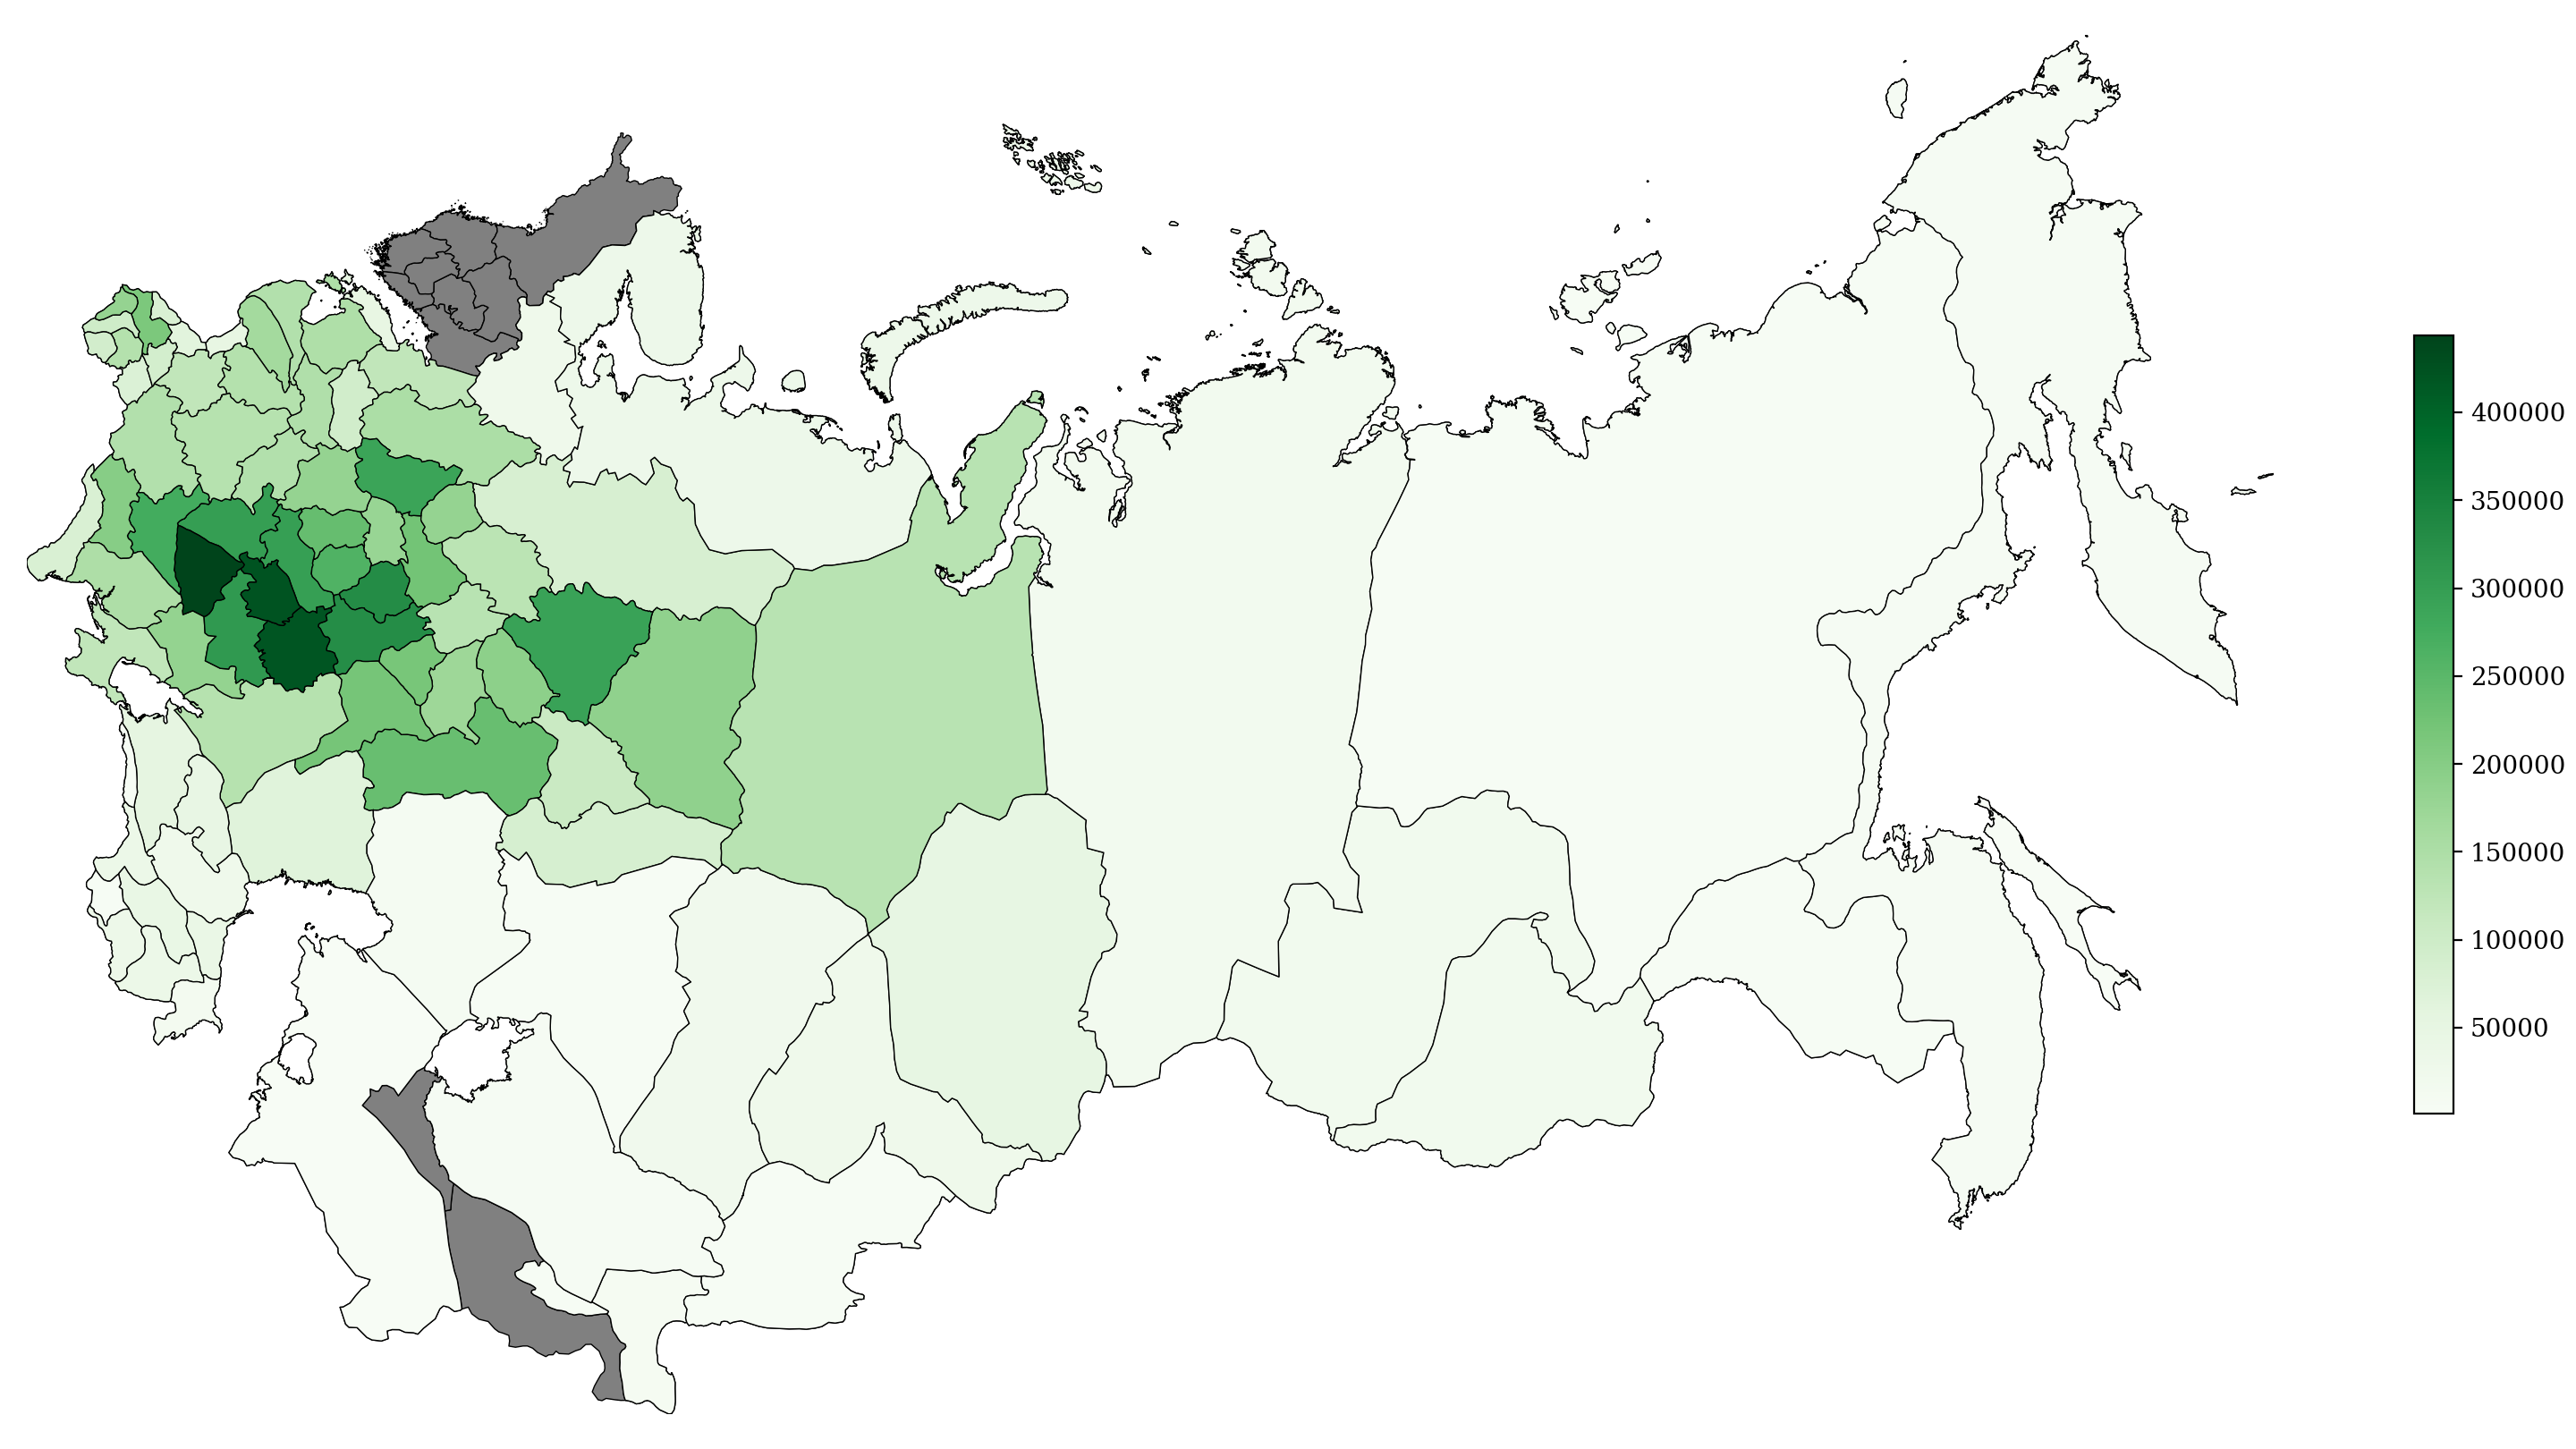
\includegraphics[height=0.9\textheight]{mig_from.png}}
}
\setbeamertemplate{navigation symbols}{}
\begin{frame}[b]{Миграция из регионов}
\hfill \href{https://russia-migrations-1897.herokuapp.com}{russia-migrations-1897.herokuapp.com}
\bigskip
\end{frame}
}

{
\usebackgroundtemplate{
  \parbox[c][\paperheight][c]{\paperwidth}{\centering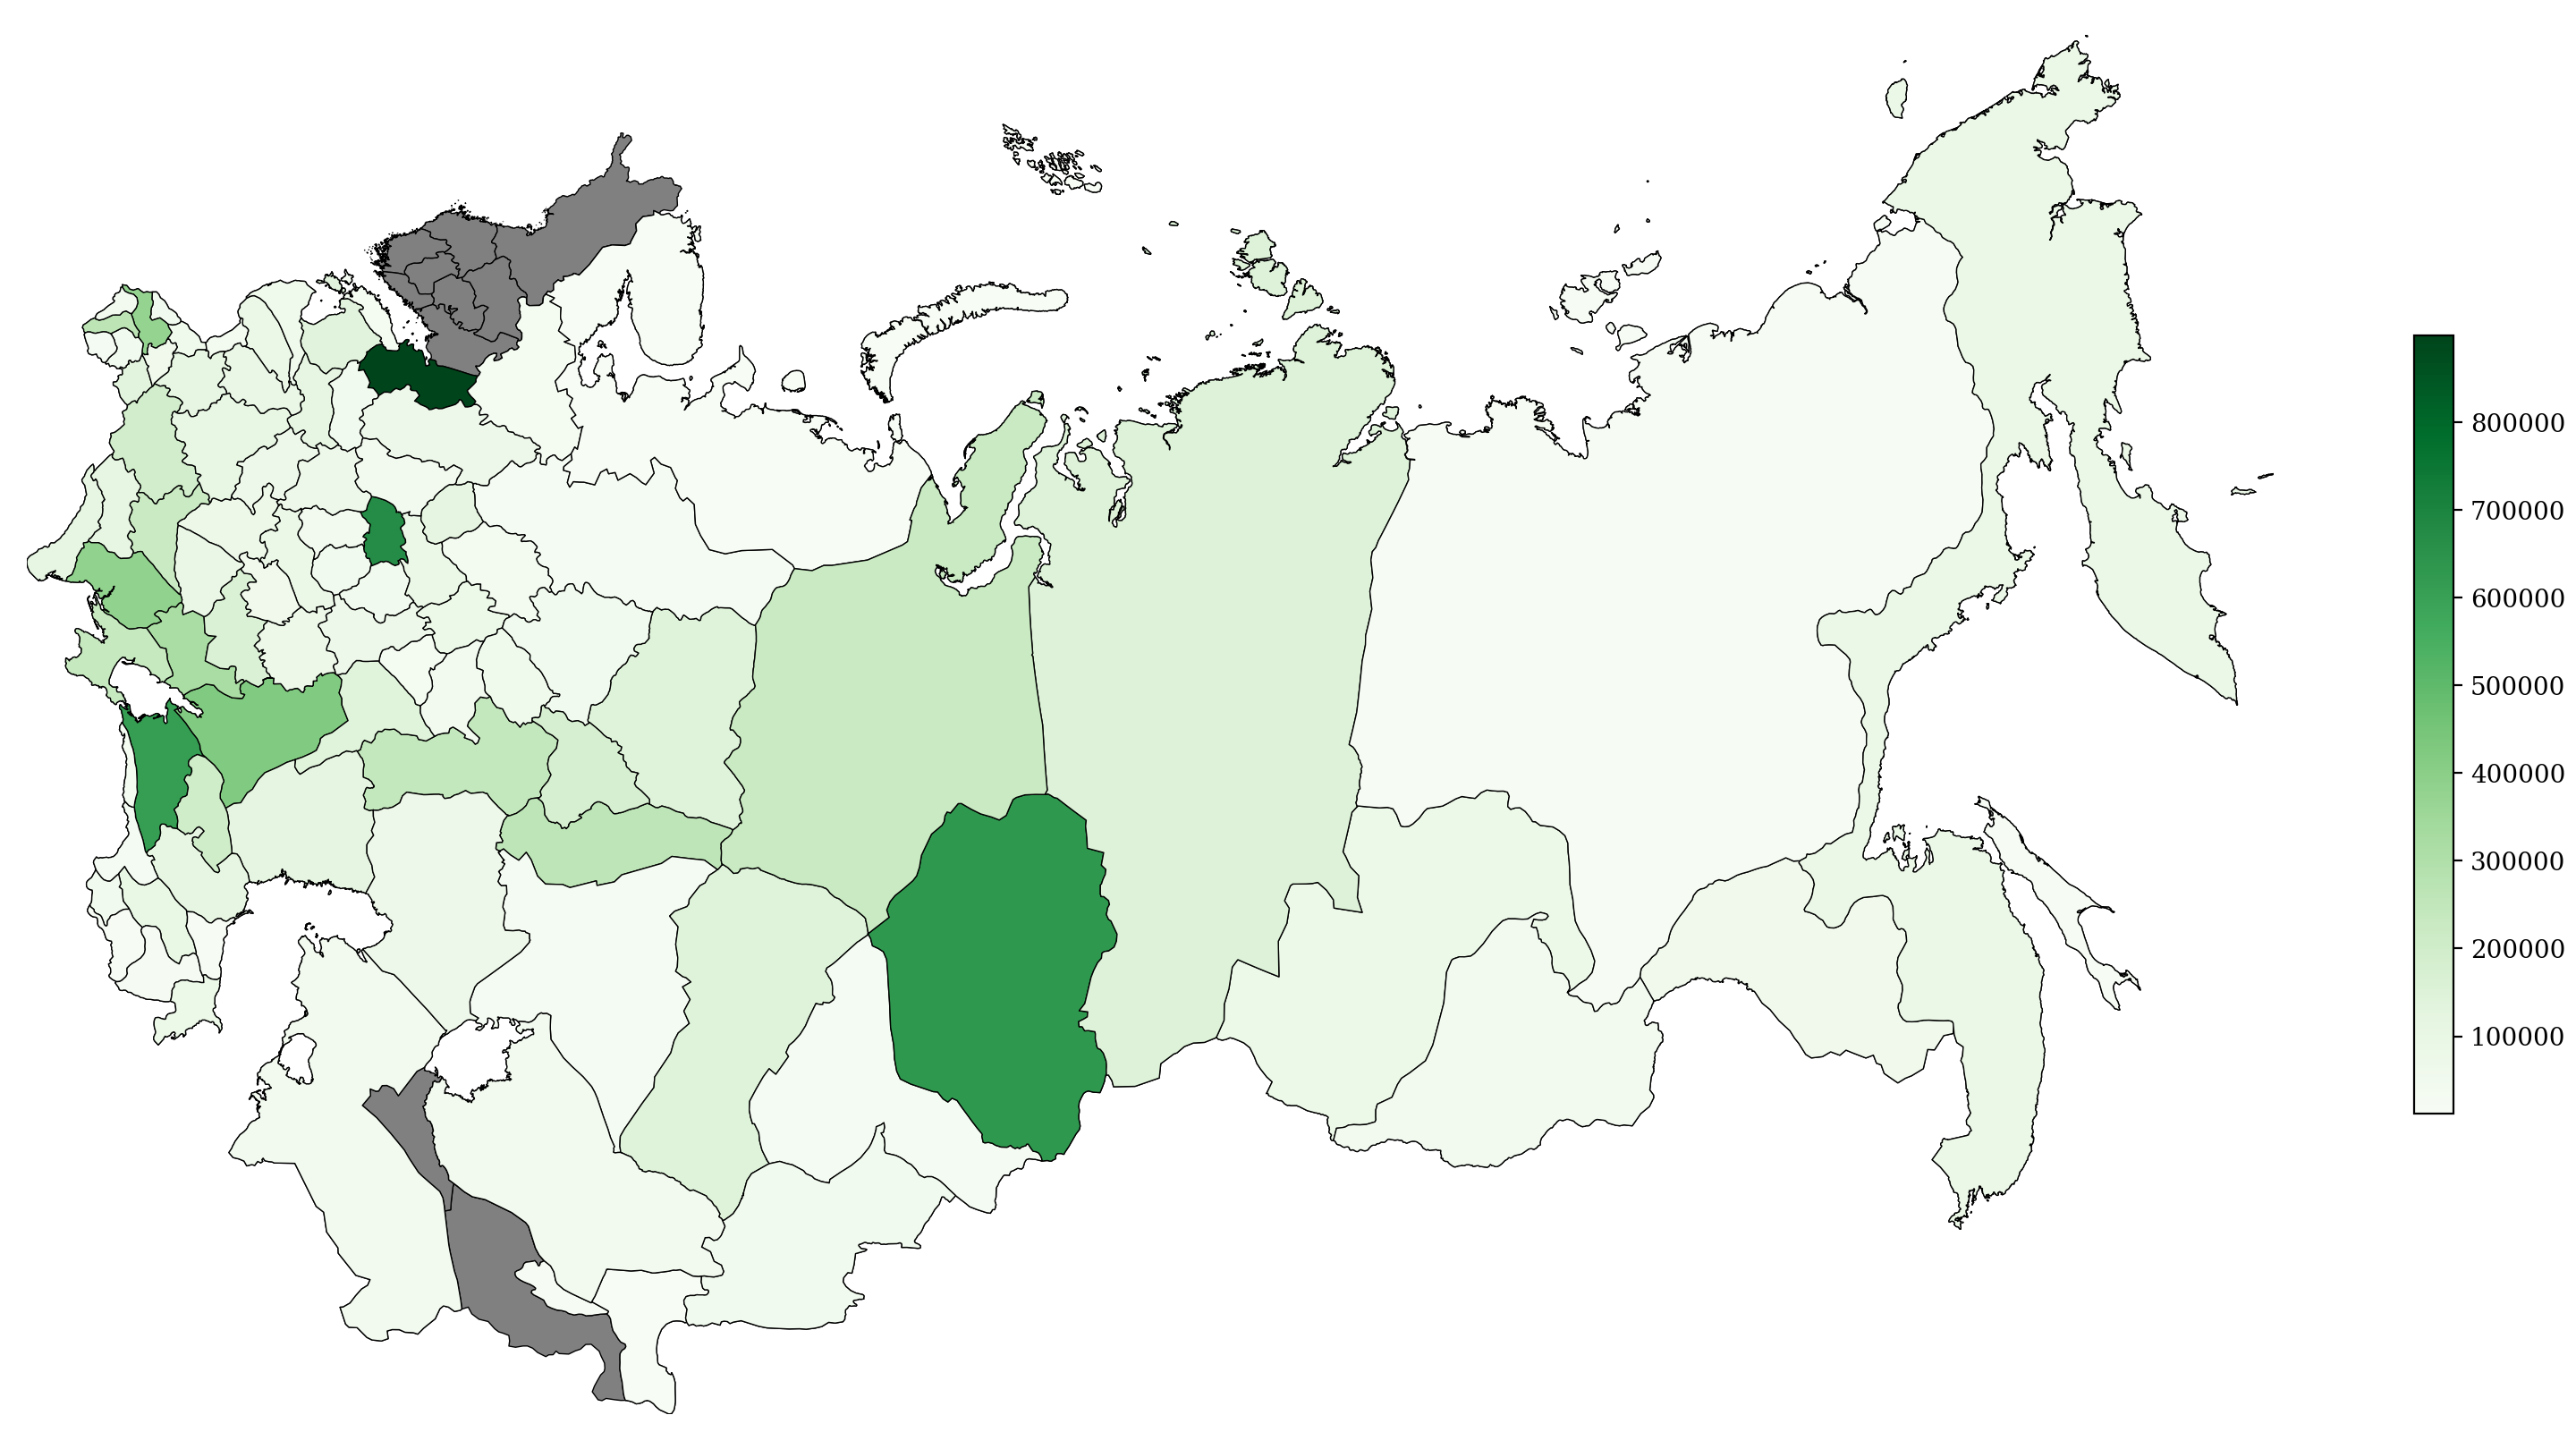
\includegraphics[height=0.9\textheight]{mig_to.png}}
}
\setbeamertemplate{navigation symbols}{}
\begin{frame}[b]{Миграция в регионы}
\hfill \href{https://russia-migrations-1897.herokuapp.com}{russia-migrations-1897.herokuapp.com}
\bigskip
\end{frame}
}

{
\usebackgroundtemplate{
  \parbox[c][\paperheight][c]{\paperwidth}{\centering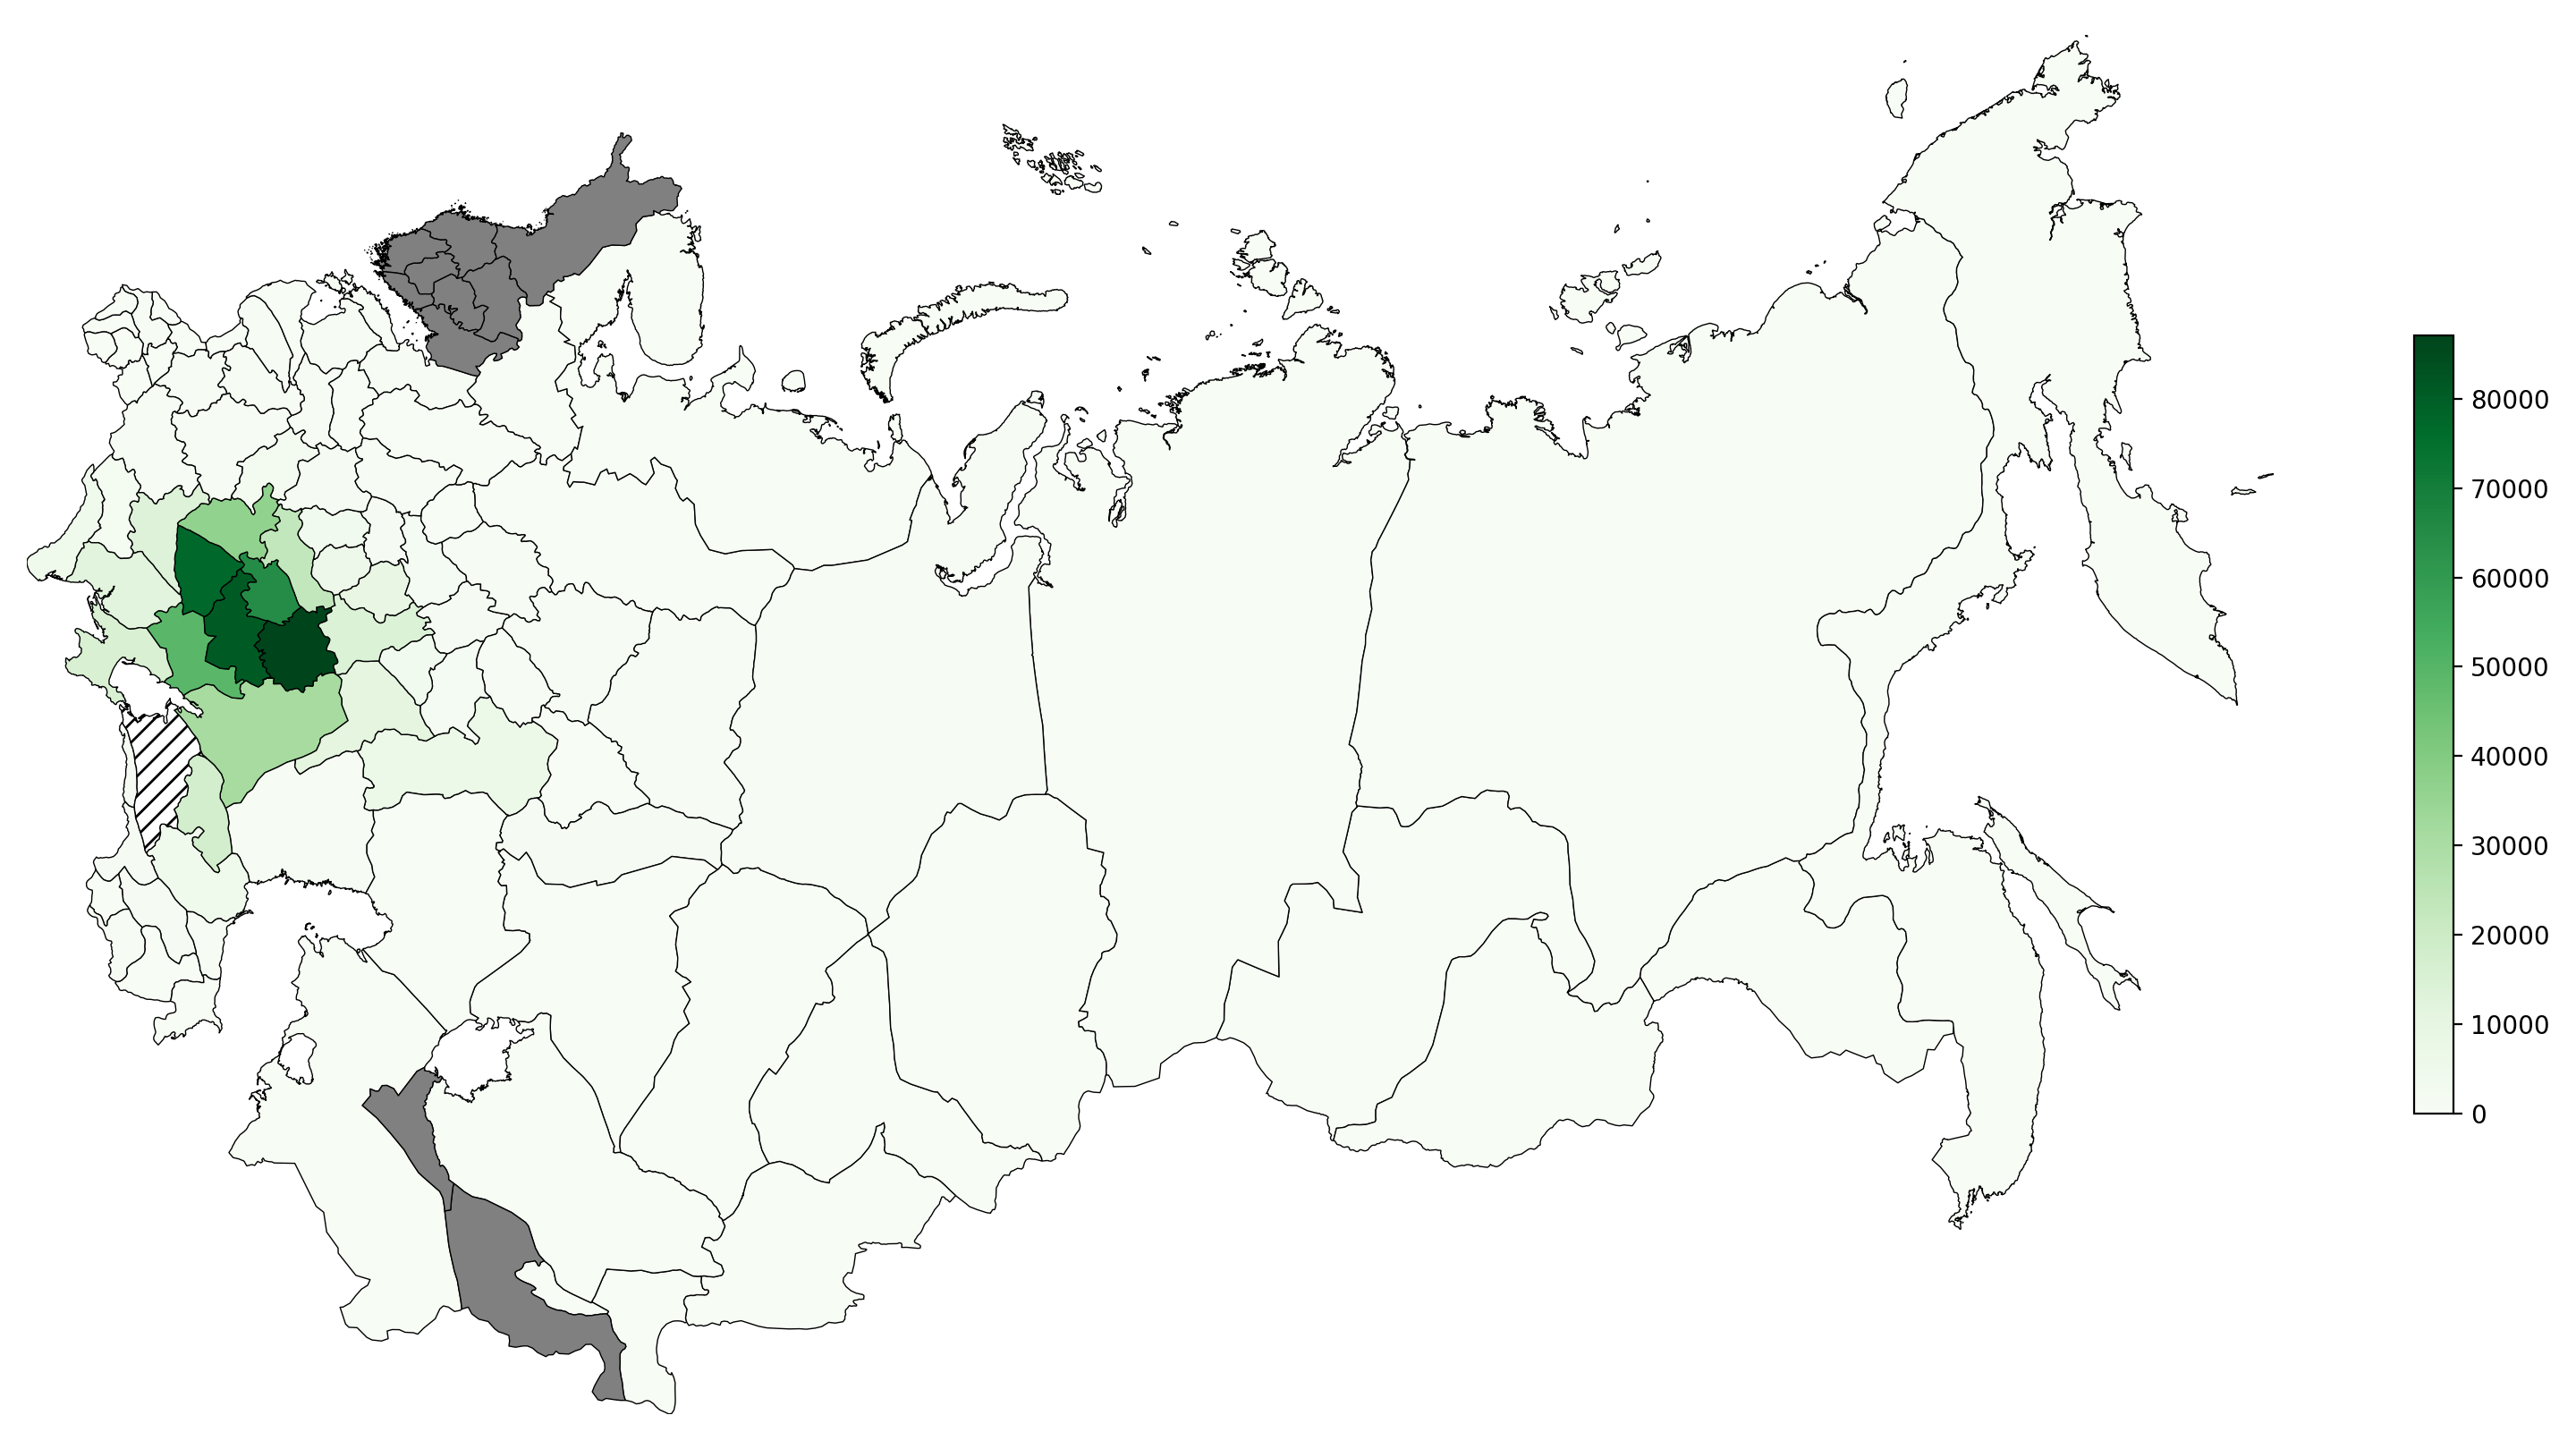
\includegraphics[height=0.9\textheight]{Kubanskaya oblast.png}}
}
\setbeamertemplate{navigation symbols}{}
\begin{frame}[b]{Миграция в Кубанскую область}
\hfill \href{https://russia-migrations-1897.herokuapp.com}{russia-migrations-1897.herokuapp.com}
\bigskip
\end{frame}
}

\section{Гравитационная модель}
\begin{frame}{Гравитационная модель}

\begin{equation*}
	M_{ij} = \beta_0 P^{\beta_1}_{i} P^{\beta_2}_{j} D^{\beta_3}_{ij} + \varepsilon_{ij}
\end{equation*}

$M_{ij}$ – число переселенцев из региона $i$ в регион $j$; $P_i$ и $P_j$ -- население региона-источника и региона-назначения, $D$ -- расстояние, $\varepsilon$ -- случайный фактор.

PPML \citep{silva_log_2006}:
\begin{gather*}
	Pr[M_{ij}] = \frac{exp(-\mu_{ij})\mu^{M_{ij}}_{ij}}{M_{ij}!},\quad M_{ij} = (0, 1, ...) \\
	\mu_{ij} = exp(\beta_0 + S_i \beta_1^T + D_{j} \beta_2^T + X_{ij} \beta_3^T)
\end{gather*}

\end{frame}

\section{Гипотезы}
\begin{frame}{Гипотезы}

\begin{columns}
	\begin{column}{0.60\textwidth}
		\begin{enumerate}
			\item На ранних этапах экономического развития, население концентрируется в крупных центрах
			\begin{equation*}
                    M_{ij} - M_{ji} = M_{ij} \left[ 1 - \frac{M_{ji}}{M_{ij}} \right] = M_{ij} \left[ 1 - \left( \frac{P_i}{P_j} \right)^{\beta_2 - \beta_1} \right]
			\end{equation*}
			Если $\beta_2>\beta_1$, $M_{ij}>M_{ij}$ \citep{poot_gravity_2016}
			\item Экономическое развитие (грамотность, выпуск промышленности) -- pull-факторы
			\item Перенаселение и низкая урбанизация -- push-факторы
		\end{enumerate}
	\end{column}
	
	\begin{column}{0.34\textwidth}
		\begin{table}
	\caption{Гипотезы}
	\label{table:hypo}
	\centering
	\begin{tabularx}{\textwidth}{XX}  %{@{}ll@{}}
		\toprule
		Переменная                   & Гипотеза                              \\ 
		\midrule
		$\textup{population}_i$, $\textup{population}_j$ & $\textup{population}_i < \textup{population}_j$ \\
		distance                     & $\approx-1$                            \\
		urbanization                 & $+$                                    \\
		density                      & $-$                                    \\
		literacy                     & $+$                                    \\
		industry                     & $+$                                    \\
		% $\Delta$climate              & $+$                                    \\
		% $\Delta$vars                 & $-$                                    \\ 
		\bottomrule
	\end{tabularx}
\end{table}
	\end{column}
\end{columns}

\end{frame}

\section{Результаты}
\begin{frame}{Результаты}
	
\begin{columns}
	\begin{column}{0.58\textwidth}
		\begin{enumerate}
			\item Все коэффициенты <<правильных>> знаков
			\item Оценка влияния населения дает смешанные результаты
			\item Более населенные регионы были источником миграции, а менее населенные -- местом назначения, однако этот эффект пропадает, если включить другие переменные
		\end{enumerate}
	\end{column}
		
	\begin{column}{0.42\textwidth}
		\begin{tiny}
			\begin{table}[htbp]\centering
\def\sym#1{\ifmmode^{#1}\else\(^{#1}\)\fi}
\caption{Основные результаты\label{table:pres}}
\begin{tabular}{l*{2}{c}}
\hline\hline
                    &\multicolumn{1}{c}{(1)}&\multicolumn{1}{c}{(2)}\\
                    &\multicolumn{1}{c}{mig\_total}&\multicolumn{1}{c}{mig\_total}\\
\hline
population\_i        &       0.927\sym{***}&       0.783\sym{***}\\
population\_j        &       0.523\sym{***}&       1.314\sym{***}\\
distance            &      -1.204\sym{***}&      -1.040\sym{***}\\
borders             &                     &       1.008\sym{***}\\
literacy\_i          &                     &       0.233\sym{**} \\
literacy\_j          &                     &       0.105         \\
urbanization\_i      &                     &     -0.0990         \\
urbanization\_j      &                     &       1.045\sym{***}\\
density\_i           &                     &       0.442\sym{***}\\
density\_j           &                     &      -0.879\sym{***}\\
industry\_share\_i    &                     &      -0.107         \\
industry\_share\_j    &                     &       0.176         \\
serfs\_i             &                     &     -0.0132         \\
serfs\_j             &                     &      -0.166\sym{***}\\
Constant            &      -5.141\sym{***}&      -11.90\sym{***}\\
\hline
Observations        &        7832         &        7656         \\
\(R^{2}\)           &       0.192         &       0.503         \\
\hline\hline
\multicolumn{3}{l}{Не показаны переменные контроля.}\\
\multicolumn{3}{l}{\sym{*} \(p<0.05\), \sym{**} \(p<0.01\), \sym{***} \(p<0.001\)}\\
\end{tabular}
\end{table}

		\end{tiny}
	\end{column}
\end{columns}
    
\end{frame}

\begin{frame}{Результаты}
	
\begin{columns}
	\begin{column}{0.58\textwidth}
		\begin{enumerate}
			\small
			\item Уровень урбанизации принимающего региона значим для всех моделей, особенно -- для миграции в города
			\item Плотность населения значима для обеих сторон взаимодействия. Это косвенно доказывает перенаселение в центральных областях
			\item Промышленность, судя по результатам, никак не влияла на внутреннюю миграцию в России, отличие от стран Европы
			\item Для мигрантов гораздо важнее демографические условия, чем присутствие еще не столь развитой промышленности
		\end{enumerate}
	\end{column}
		
	\begin{column}{0.42\textwidth}
		\begin{tiny}
			\begin{table}[htbp]\centering
\def\sym#1{\ifmmode^{#1}\else\(^{#1}\)\fi}
\caption{Города-Уезды\label{table:r-u}}
\begin{tabular}{l*{2}{c}}
\hline\hline
                    &\multicolumn{1}{c}{(1)}&\multicolumn{1}{c}{(2)}\\
                    &\multicolumn{1}{c}{mig\_rural}&\multicolumn{1}{c}{mig\_urban}\\
\hline
population\_i        &       0.841\sym{***}&       0.801\sym{***}\\
population\_j        &       1.339\sym{***}&       1.182\sym{***}\\
distance            &      -0.940\sym{***}&      -1.170\sym{***}\\
borders             &       1.342\sym{***}&       0.654\sym{***}\\
literacy\_i          &       0.131         &       0.267\sym{**} \\
literacy\_j          &       0.171         &     0.00894         \\
urbanization\_i      &     -0.0344         &      -0.141         \\
urbanization\_j      &       0.368\sym{**} &       1.929\sym{***}\\
density\_i           &       0.708\sym{***}&       0.177\sym{*}  \\
density\_j           &      -1.087\sym{***}&      -0.595\sym{***}\\
industry\_share\_i    &      -0.255         &      0.0969         \\
industry\_share\_j    &       0.432\sym{***}&      -0.207         \\
serfs\_i             &     0.00709         &     -0.0613         \\
serfs\_j             &      -0.180\sym{***}&     -0.0729\sym{***}\\
Constant            &      -15.79\sym{***}&      -9.009\sym{***}\\
\hline
Observations        &        7656         &        7656         \\
\(R^{2}\)           &       0.323         &       0.576         \\
\hline\hline
\multicolumn{3}{l}{Не показаны переменные контроля.}\\
\multicolumn{3}{l}{\sym{*} \(p<0.05\), \sym{**} \(p<0.01\), \sym{***} \(p<0.001\)}\\
\end{tabular}
\end{table}

		\end{tiny}
	\end{column}
\end{columns}
	
\end{frame}


\section{Заключение}
\begin{frame}{Заключение}
	
Дальнейшее развитие темы:
	
\begin{itemize}
	\item Добавление новых переменных: они существуют, но их трудно добыть 
	\item Решение проблемы эндогенности
	\item Более интересный исследовательский вопрос
\end{itemize}

\end{frame}

\begin{frame}[shrink=20]{Список литературы}
    \printbibliography
\end{frame}

\section{Приложение}
\begin{frame}{Спасибо за внимание!}
    \begin{itemize}
	    \item \href{https://russia-migrations-1897.herokuapp.com}{Карты для некоторых переменных}
	    \item \href{https://github.com/fant0md/empire-migrations-coursework}{Репозиторий с текстом работы, данными и кодом}
    \end{itemize}
\end{frame}

\end{document}
